\part{Kinematics}
\label{partKinematics}

The irregular dodecahedron used here as a model for alveoli describes a 3D structure composed of thirty 1D rods (the septal chords) joined at twenty nodes (the vertices) that collectively circumscribe twelve 2D pentagonal membranes (the alveolar septa) that in turn envelop an alveolar sac whose volume is represented using sixty tetrahedra.  To be able to describe the overall mechanical response of this 3D dodecahedral structure, it is conjectured to be sufficient to know the individual mechanical responses of its 1D septal chords, its 2D septal membranes, and the 3D void within.  Their relevant kinematics are presented here, along with the shape functions used for interpolation and our description of deformation.

\section{1D Chords}

The stretch of a rod under extension is a ratio of its lengths.  Specifically, $\lambda \defeq L / L_0$ where $L$ and $L_0$ are its current and reference lengths, respectively, whose strain and strain rate are taken to be $e = \ln \lambda$ and $\mathrm{d} e = \lambda^{-1} \mathrm{d} \lambda$.  This is often referred to as a logarithmic, natural or true strain.  Consequently, the kinematic analysis of a chord is trivial.

\subsection{Shape Functions for Interpolating a Rod}

A two-noded alveolar chord has shape functions $N_i$, $i=1,2$, that, when evaluated in its natural coordinate system where $-1 \leq \xi \leq 1$, describe a matrix with elements
\begin{subequations}
    \begin{align}
\mathbf{N} & = \begin{bmatrix} N_1 & N_2 \end{bmatrix} =
\begin{bmatrix}
\frac{1}{2} \, (1 - \xi) &  \frac{1}{2} \, (1 + \xi)
\end{bmatrix} \\
\intertext{that interpolate vector fields according to}
\mathbfit{x} ( \xi ) & = \sum_{i=1}^2 N_i ( \xi ) \, x_i , \quad
\mathbfit{u} ( \xi ) = \sum_{i=1}^2 N_i ( \xi ) \, u_i  \\
\intertext{etc., and whose spatial gradients are} 
N_{1,\xi} & = -\tfrac{1}{2} 
\quad \text{and} \quad
N_{2,\xi} = \tfrac{1}{2}
\end{align}
\end{subequations}
wherein $\xi$ is the natural co-ordinate.  Components $x_i$ and $u_i \defeq x_i - x_{0i}$ are their global co-ordinates and displacements, respectively, located at the two nodes of a chord evaluated in the co-ordinate frame $( \vec{\mathbfsf{e}}_1 , \vec{\mathbfsf{e}}_2 , \vec{\mathbfsf{e}}_3 )$ of Fig.~\ref{figchord} with the chordal axis lying in the $\vec{\mathbfsf{e}}_1$ direction.

\subsection{Deformation Gradient for a Rod}

The deformation gradient in this case is simply
\begin{equation}
    \mathbfsf{F} ( \xi ) = 1 + \frac{\partial \mathbfit{u}}{\partial \xi} 
    \left( \frac{\partial \mathbfit{x}_0 }{\partial \xi} \right)^{-1} = 
    1 + \sum_{i=1}^2 N_{i,\xi} u_i \left( \sum_{i=1}^2 N_{i,\xi} x_{0i} \right)^{-1} = 
    1 + \frac{u_2 - u_1}{x_{02} - x_{01}} = \frac{x_2 - x_1}{x_{02} - x_{01}}
\end{equation}
which is uniform over the length of a chord, i.e., it is independent of $\xi$.

\section{2D Triangles}

Triangular elements are needed in a support capacity in order to construct our alevolar model; specifically, the four surfaces of a tetrahedron are triangles.  What is required of them is a capability to compute the traction acting across such a surface through integration.  This requires knowledge of their shape functions and quadrature rules, the latter of which is discussed in \S\ref{partNumericalMethods}. 

The shape functions for a triangle expressed in terms of its natural co-ordinates $( \xi , \eta )$, where $0 \leq \xi \leq 1$ and $0 \leq \eta \leq \xi$, are given by
\begin{subequations}
    \label{triangleShapeFns}
    \begin{align}
    N_1 & = 1 - \xi - \eta &
    N_2 & = \xi &
    N_3 & = \eta 
    \intertext{with gradients of}
    N_{1,\xi} & = -1 & N_{2,\xi} & = 1 & N_{3,\xi} & = 0 \\
    N_{2,\eta} & = -1 & N_{2,\eta} & = 0 & N_{3,\eta} & = 1
    \end{align}
\end{subequations}
so that the area of a triangle in its natural co-ordinates is \textfrac{1}{2}.  

No further kinematics are required from triangular elements in our analysis.

\section{2D Irregular Pentagons}

The kinematics of an irregular pentagon, on the other hand, are not trivial.  Shape functions are required from which deformation gradients can then be constructed.  Once a deformation gradient is in hand, the state of stretch occurring within a pentagon can finally be derived.  Several possible decompositions of the deformation gradient are possible, i.e., stretch is not unique in 2D (nor in 3D).  Here we employ the Laplace stretch \cite{Freedetal19}.

\subsection{Wachspress' Shape Functions for Interpolating an Irregular Pentagon}
\label{secShapeFns}

In 1975, Wachspress \cite{Wachspress75,Wachspress16} derived a set of shape functions $N_i$ that are capable of interpolating convex polyhedra.  His shape functions take on the form of rational polynomials, viz., $N_i = A_i / B$ where $A_i$ and $B$ are polynomials.  In contrast, classic isoparametric elements are constructed from polynomial shape functions \cite{Hughes87}.  For the Wachspress shape functions of a pentagon, the $A_i$ are cubic polynomials, while $B$ is a quadratic polynomial.

Let us consider a convex pentagonal domain $\Omega$ defined over $\mathbb{R}^2$ whose vertices have global co-ordinates of
\begin{displaymath}
(x_1, y_1) , \; (x_2, y_2) , \; (x_3, y_3) , \; (x_4, y_4), \; (x_5, y_5)
\end{displaymath}
when evaluated in the pentagonal co-ordinate system $( \vec{\mathbfsf{e}}_1 , \vec{\mathbfsf{e}}_2 )$ of Fig.~\ref{figPentagonCoord}, with $\vec{\mathbfsf{e}}_3$ being an outward normal to the pentagon.  Associated with this set of global co-ordinates is a set of local or natural co-ordinates
\begin{displaymath}
(\xi_1 , \eta_1) , \; (\xi_2 , \eta_2) , \; (\xi_3 , \eta_3) , \; (\xi_4 , \eta_4) , \; (\xi_5 , \eta_5)
\end{displaymath}
that describe a mapping or interpolation of
\begin{equation}
\begin{aligned}
x(\xi, \eta) & = \sum\nolimits_{i=1}^5 N_i (\xi, \eta) \, x_i \\
y(\xi, \eta) & = \sum\nolimits_{i=1}^5 N_i (\xi, \eta) \, y_i
\end{aligned} 
\qquad \text{or} \qquad
\mathbfit{x}(\boldsymbol{\xi}) = \sum_{i=1}^5 N_i (\boldsymbol{\xi}) \, 
\mathbfit{x}_{\,i}
\end{equation}
which relate natural co-ordinates $\boldsymbol{\xi} \equiv (\xi, \eta)$ to global co-ordinates $\mathbfit{x} \equiv (x, y)$, where $\mathbfit{x}_{\,i} \equiv (x_i, y_i)$ are nodal co-ordinates at the $i^{\mathrm{th}}$ vertex, with $i$ indexing counterclockwise around a pentagon according to Fig.~\ref{figRegPentagon}.  Displacement $\mathbfit{u} (\mathbfit{x}) \defeq \mathbfit{x} - \mathbfit{x}_0$, with reference co-ordinates $\mathbfit{x}_0 \equiv (x_0, y_0)$, also obeys this mapping
\begin{equation}
\begin{aligned}
u(\xi, \eta) & = \sum\nolimits_{i=1}^5 N_i (\xi, \eta) \, u_i \\
v(\xi, \eta) & = \sum\nolimits_{i=1}^5 N_i (\xi, \eta) \, v_i
\end{aligned} 
\qquad \text{or} \qquad
\mathbfit{u}(\boldsymbol{\xi}) = \sum_{i=1}^5 N_i (\boldsymbol{\xi}) \, 
\mathbfit{u}_{\,i}
\end{equation}
whose co-ordinates $\mathbfit{u}_{\,i} \equiv (u_i , v_i)$ designate the nodal displacements.

Shape functions $N_i (\boldsymbol{\xi}) \equiv N_i (\xi, \eta)$ are interpolation functions that place any position $P$ with local co-ordinates $\boldsymbol{\xi} \equiv (\xi, \eta) \in \widebar{\Omega}$, where $\widebar{\Omega} \defeq \Omega \cup \partial\Omega$, into their global co-ordinates $\mathbfit{x} \equiv (x,y)$.  The shape functions of Wachspress \cite{Wachspress75,Wachspress16} possess the following properties \cite{SukumarMalsch06}:
\begin{enumerate}
	\item Partition of unity: $\sum\nolimits_{i=1}^5 N_i (\boldsymbol{\xi}) = 1$, \; $0 \leq N_i (\boldsymbol{\xi}) \leq 1$.
	\item Interpolate nodal data: $N_i (\boldsymbol{\xi}_{\,j}) = \Xi_{ij}$.
	\item Linear completeness: $\sum\nolimits_{i=1}^5 N_i (\boldsymbol{\xi}) \, \mathbfit{x}_{\,i} = \mathbfit{x}$.
	\item For $\boldsymbol{\xi} \in \Omega$, $N_i (\boldsymbol{\xi})$ is $C^{\infty}$, but for $\boldsymbol{\xi} \in \partial \Omega$, $N_i (\boldsymbol{\xi})$ is $C^0$, i.e., interpolation is linear along an edge (or chord) connecting two neighboring vertices. 
\end{enumerate}

For interpolating a convex, planar, pentagonal shape, the shape functions of Wachspress have polynomials of order three in their numerators, and another polynomial of order two in their denominators; specifically, we write them here as
\begin{subequations}
	\label{shapeFunctions}
	\begin{align}
	N_{i+1} (\xi, \eta) & = \kappa_i \, A_i (\xi, \eta) / B(\xi, \eta) , 
	\qquad i = 1, 2 , \dots , 5 \\ 
	\intertext{with scaling factors $\kappa_i$, where $N_1 \Leftarrow N_6$, whose numerators and denominator for interpolating a pentagon are evaluated via}
	A_i (\xi, \eta) & = \alpha_{0i} + \alpha_{1i} \xi + \alpha_{2i} \eta + 
	\alpha_{3i} \xi^2 + \alpha_{4i} \xi\eta + \alpha_{5i} \eta^2 \notag \\ 
	\mbox{} & \phantom{\mbox{} = \alpha_{0i}} + \alpha_{6i} \xi^3 + 
	\alpha_{7i} \xi^2 \eta + \alpha_{8i} \xi \eta^2 + \alpha_{9i} \eta^3
	\label{shapeFnNum} \\
	B (\xi, \eta) & = \beta_0 + \beta_1 \xi + \beta_2 \eta + \beta_3 \xi^2 + 
	\beta_4 \xi\eta + \beta_5 \eta^2 
	\label{shapeFnDenom}
	\end{align}
\end{subequations}
where coefficients in the numerator, i.e., $A_i$, differ with index $i$, while those in the denominator, viz., $B \defeq \sum_{i=1}^5 A_i$, are the same for all five shape functions.  

We apply the construction technique of Dasgupta \cite{Dasgupta03} to compute the shape functions of Wachspress for an irregular convex pentagon.  Consider a chord $c_i$ that connects vertex $\mathbfit{\xi}_{\,i-1} = (\xi_{i-1} , \eta_{i-1})$ with vertex $\mathbfit{\xi}_{\,i} = (\xi_i , \eta_i)$ via a straight line segment such that $\ell_i = 0$ with $\ell_i \defeq 1 - a_{i} \xi - b_i \eta$ wherein
\begin{subequations}
	\begin{align}
	a_i & = \frac{\eta_i - \eta_{i-1}}{\xi_{i-1} \eta_i - \xi_i \eta_{i-1}} \\
	b_i & = \frac{\xi_{i-1} - \xi_i}{\xi_{i-1} \eta_i - \xi_i \eta_{i-1}} \\
	\intertext{for which Dasgupta derived the following set of constraints}
	\kappa_i & = \kappa_{i-1} \left( 
	\frac{a_{i+1} (\xi_{i-1} - \xi_i) + b_{i+1} (\eta_{i-1} - \eta_i)}
	{a_{i-1} (\xi_i - \xi_{i-1}) + b_{i-1} (\eta_i - \eta_{i-1})} \right) 
	\end{align}
\end{subequations}
with recursion starting at $\kappa_1 \defeq 1$.  Coefficients $\kappa_i$ enforce property 4 listed above.

With this information in hand, we derived the rational polynomials describing Wachspress' shape functions for a pentagon specified in Eq.~(\ref{shapeFunctions}) in terms of parameters $a_i$, $b_i$ and $\kappa_i$.  The polynomial coefficients for the $A_i$ in Eq.~(\ref{shapeFnNum}) have values of
\begin{subequations}
	\label{shapeFnCoefs}
	\begin{align}
	\alpha_{0i} & = 1 \\
	\alpha_{1i} & = -( a_{i+1} + a_{i+2} + a_{i+3} ) \\
	\alpha_{2i} & = -( b_{i+1} + b_{i+2} + b_{i+3} ) \\
	\alpha_{3i} & = a_{i+1} a_{i+2} + a_{i+2} a_{i+3} + a_{i+3} a_{i+1} \\
	\alpha_{4i} & = a_{i+1} ( b_{i+2} + b_{i+3} ) + a_{i+2} ( b_{i+1} + 
	b_{i+3} ) + a_{i+3} ( b_{i+1} + b_{i+2} ) \\
	\alpha_{5i} & = b_{i+1} b_{i+2} + b_{i+2} b_{i+3} + b_{i+3} b_{i+1} \\
	\alpha_{6i} & = -a_{i+1} a_{i+2} a_{i+3} \\
	\alpha_{7i} & = -( a_{i+1} a_{i+2} b_{i+3} + a_{i+1} b_{i+2} a_{i+3} + 
	b_{i+1} a_{i+2} a_{i+3} ) \\
	\alpha_{8i} & = -( a_{i+1} b_{i+2} b_{i+3} + b_{i+1} a_{i+2} b_{i+3} + 
	b_{i+1} b_{i+2} a_{i+3} ) \\
	\alpha_{9i} & = -b_{i+1} b_{i+2} b_{i+3}
	\end{align}
\end{subequations}
which differ for each shape function via index $i = 1,2,\dots,5$, while the polynomial coefficients for $B$ in Eq.~(\ref{shapeFnDenom}) have values of
\begin{equation}
\beta_i = \sum_{j=1}^5 \alpha_{ij} \kappa_j, \qquad i = 0, 1, \dots, 5
\end{equation}
which are the same for all five shape functions.  Sums over the four cubic terms in Eq.~(\ref{shapeFnCoefs}) all vanish---a byproduct of Wachpress' formulation.  In the above formul\ae, an index count of $i \equiv 0 \implies i = 5$, while index counts of $i \equiv 6 \implies i = 1$, $i \equiv 7 \implies i = 2$ and $i \equiv 8 \implies i = 3$.  Shape function $N_1$ is illustrated in Fig.~\ref{figShapeFuntion}, with like images applying for the other four shape functions.

\begin{figure}
	\centering
	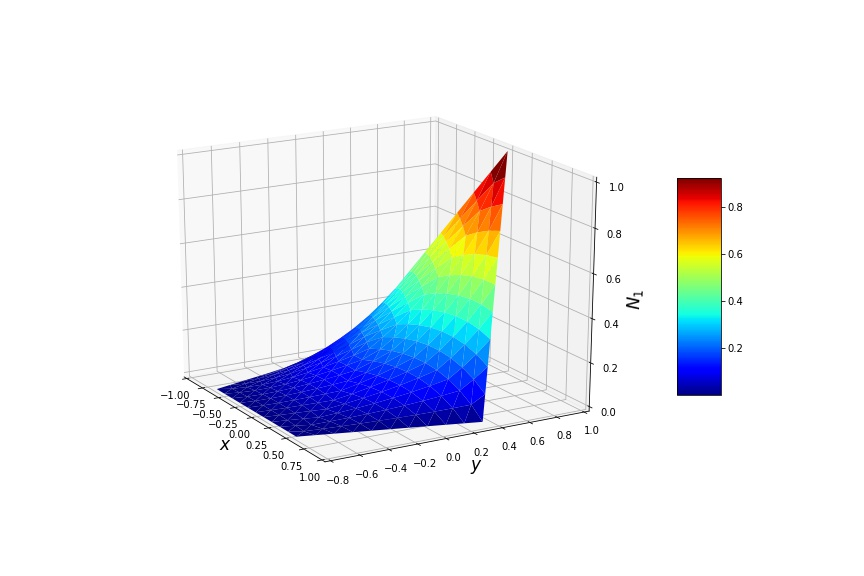
\includegraphics[width=0.9\textwidth]{figures/shapeFunction.jpg}
	\caption{Wachspress shape functions for a pentagon, in this case, shape function $N_1$.}
	\label{figShapeFuntion}
\end{figure}

\subsection{Spatial Derivatives of Shape Functions}

The first derivatives of Wachspress' shape functions for a pentagon are
\begin{subequations}
    \label{shapeFunctionGradients}
	\begin{align}
	N_{i+1,\xi} (\xi, \eta) & = \kappa_i \, \mathcal{N}_{i,\xi}(\xi, \eta) /
	B^2(\xi, \eta) \\
	N_{i+1,\eta} (\xi, \eta) & = \kappa_i \, \mathcal{N}_{i,\eta}(\xi, \eta) /
	B^2(\xi, \eta) \\
	\intertext{where $N_{i+1,\xi}  (\xi, \eta) = \partial N_{i+1} (\xi, \eta) / \partial \xi$ and $N_{i+1,\eta} (\xi, \eta) = \partial N_{i+1} (\xi, \eta) / \partial \eta$ with}
	\mathcal{N}_{i,\xi} (\xi,\eta) & = B(\xi, \eta) A_{i,\xi} (\xi, \eta) -
	B_{,\xi} (\xi, \eta) A_i (\xi, \eta) \\
	\mathcal{N}_{i,\eta} (\xi,\eta) & = B(\xi, \eta) A_{i,\eta} (\xi, \eta) - 
	B_{,\eta} (\xi, \eta) A_i (\xi, \eta) \\
	\intertext{which contain the polynomials}
	A_{i,\xi} (\xi, \eta) & = \alpha_{1i} + 2 \alpha_{3i} \xi + \alpha_{4i} \eta +
	3 \alpha_{6i} \xi^2 + 2 \alpha_{7i} \xi \eta + \alpha_{8i} \eta^2
	\label{shapeFnGradXiNum} \\
	A_{i,\eta} (\xi, \eta) & = \alpha_{2i} + \alpha_{4i} \xi + 2 \alpha_{5i} \eta + 
	\alpha_{7i} \xi^2 + 2 \alpha_{8i} \xi\eta + 3 \alpha_{9i} \eta^2 
	\label{shapeFnGradEtaNum} \\
	B_{,\xi} (\xi, \eta) & = \beta_1 + 2 \beta_3 \xi + \beta_4 \eta
	\label{shapeFnGradXiDenom} \\
	B_{,\eta} (\xi, \eta) & = \beta_2 + \beta_4 \xi + 2 \beta_5 \eta 
	\label{shapeFnGradEtaDenom}
	\end{align}
\end{subequations}
from which the deformation and displacement gradients are constructed.

The second derivatives of these shape functions, which we used to test the compatibility conditions of this element, are described by
\begin{subequations}
	\begin{align}
	N_{i+1,\xi\xi} & = \kappa_i \, \mathfrak{N}_{i,\xi\xi}(\xi,\eta) /
	B^3 (\xi,\eta) \\
	N_{i+1,\xi\eta} & = \kappa_i \, \mathfrak{N}_{i,\xi\eta}(\xi,\eta) /
	B^3(\xi,\eta) \\
	N_{i+1,\eta\xi} & = \kappa_i \, \mathfrak{N}_{i,\eta\xi}(\xi,\eta) /
	B^3(\xi,\eta) \\
	N_{i+1,\eta\eta} & = \kappa_i \, \mathfrak{N}_{i,\eta\eta}(\xi,\eta) /
	B^3(\xi,\eta) \\
	\intertext{where $N_{i+1,\xi\eta}  (\xi, \eta) = \partial^2 N_{i+1} (\xi, \eta) / \partial \xi \partial \eta$, etc., and  where}
	\mathfrak{N}_{i,\xi\xi} (\xi,\eta) & = B(\xi,\eta)
	\mathcal{N}_{i,\xi\xi} (\xi,\eta) - 2 B_{,\xi} (\xi,\eta) 
	\mathcal{N}_{i,\xi} (\xi,\eta) \\
	\mathfrak{N}_{i,\xi\eta}  (\xi,\eta)& = B(\xi,\eta) 
	\mathcal{N}_{i,\xi\eta} (\xi,\eta) - 2 B_{,\xi} (\xi,\eta) 
	\mathcal{N}_{i,\eta} (\xi,\eta) \\
	\mathfrak{N}_{i,\eta\xi}  (\xi,\eta)& = B(\xi,\eta)
	\mathcal{N}_{i,\eta\xi} (\xi,\eta) - 2 B_{,\eta} (\xi,\eta) 
	\mathcal{N}_{i,\xi} (\xi,\eta) \\
	\mathfrak{N}_{i,\eta\eta} (\xi,\eta) & = B(\xi,\eta) 
	\mathcal{N}_{i,\eta\eta} (\xi,\eta) - 2 B_{,\eta} (\xi,\eta) 
	\mathcal{N}_{i,\eta} (\xi,\eta) \\
	\intertext{wherein}
	\mathcal{N}_{i,\xi\xi} (\xi,\eta) & = B(\xi,\eta) A_{i,\xi\xi} (\xi,\eta) -
	B_{,\xi\xi} (\xi\eta) A_{i} (\xi\eta) \\
	\mathcal{N}_{i,\xi\eta} (\xi,\eta) & = B (\xi,\eta) A_{i,\xi\eta} (\xi,\eta) +
	B_{,\xi} (\xi,\eta) A_{i,\eta} (\xi,\eta) \notag \\
	\mbox{} & - B_{,\eta} (\xi,\eta) A_{i,\xi} (\xi,\eta) - 
	B_{,\xi\eta} (\xi,\eta) A_i (\xi,\eta) \\
	\mathcal{N}_{i,\eta\xi} (\xi,\eta) & = B (\xi,\eta) A_{i,\eta\xi} (\xi,\eta) +
	B_{,\eta} (\xi,\eta) A_{i,\xi} (\xi,\eta) \notag \\
	\mbox{} & - B_{,\xi} (\xi,\eta) A_{i,\eta} (\xi,\eta) - 
	B_{,\eta\xi} (\xi,\eta) A_i (\xi,\eta)  \\
	\mathcal{N}_{i,\eta\eta} (\xi,\eta) & = B(\xi,\eta) A_{i,\eta\eta} (\xi,\eta) -
	B_{,\eta\eta} (\xi,\eta) A_{i} (\xi,\eta) \\
	\intertext{which contain polynomials}
	A_{i,\xi\xi} (\xi,\eta) & = 2 \alpha_{3i} + 6 \alpha_{6i} \xi + 2 \alpha_{7i} \eta \\
	A_{i,\xi\eta} (\xi,\eta) & = \alpha_{4i} + 2 \alpha_{7i} \xi + 2 \alpha_{8i} \eta \\
	A_{i,\eta\eta} (\xi,\eta) & = 2 \alpha_{5i} + 2 \alpha_{8i} \xi + 6 \alpha_{9i} \eta \\
	B_{,\xi\xi} (\xi,\eta) & = 2 \beta_3 \\
	B_{,\xi\eta} (\xi,\eta) & = \beta_4 \\
	B_{,\eta\eta} (\xi,\eta) & = 2 \beta_5
	\end{align}
\end{subequations}
with $A_{i,\xi\eta} (\xi,\eta) = A_{i,\eta\xi} (\xi,\eta)$ and $B_{,\xi\eta} (\xi,\eta) = B_{,\eta\xi} (\xi,\eta)$. 

\subsection{Deformation Gradient for an Irregular Pentagon}

Derivatives of displacement $(u, v)$ taken with respect to the local co-ordinates $(\xi, \eta)$ used to describe the shape functions $N_i (\xi, \eta)$ of a pentagon result in a local displacement gradient with components
\begin{subequations}
	\label{gradient}
	\begin{align}
	\begin{bmatrix}
	\partial u / \partial\xi & \partial u / \partial\eta \\
	\partial v / \partial\xi & \partial v / \partial\eta
	\end{bmatrix} & = 
	\begin{bmatrix}
	\sum\nolimits_{i=1}^5 N_{i,\xi} (\xi,\eta) \, u_i & \sum\nolimits_{i=1}^5 N_{i,\eta} (\xi,\eta) \, u_i \\
	\sum\nolimits_{i=1}^5 N_{i,\xi} (\xi,\eta) \, v_i & \sum\nolimits_{i=1}^5 N_{i,\eta} (\xi,\eta) \, v_i
	\end{bmatrix} 
	\label{displacementGradients} \\
	\intertext{where $u \defeq x - x_0$ and $v \defeq y - y_0$.  Gradients of the global co-ordinates $(x_0,y_0)$ evaluated in a reference state taken with respect to local co-ordinates $(\xi, \eta)$ are described by the matrix equation} 
	\begin{bmatrix}
	\partial x_0 / \partial\xi & \partial x_0 / \partial\eta \\
	\partial y_0 / \partial\xi & \partial y_0 / \partial\eta
	\end{bmatrix} & = 
	\begin{bmatrix}
	\sum\nolimits_{i=1}^5 N_{i,\xi} (\xi,\eta) \, x_{0i} & \sum\nolimits_{i=1}^5 N_{i,\eta} (\xi,\eta) \, x_{0i} \\
	\sum\nolimits_{i=1}^5 N_{i,\xi} (\xi,\eta) \, y_{0i} & \sum\nolimits_{i=1}^5 N_{i,\eta} (\xi,\eta) \, y_{0i}
	\end{bmatrix}
	\label{co-ordinateGradients} \\
	\intertext{wherein $(x_{0i}, y_{0i})$ are the reference global co-ordinates at the $i^{\mathrm{th}}$ vertex, while gradients of the global co-ordinates $(x,y)$ evaluated in the current state taken with respect to local co-ordinates $(\xi, \eta)$ are described by the matrix equation}
	\mathbf{J} \defeq \begin{bmatrix}
	\partial x / \partial\xi & \partial x / \partial\eta \\
	\partial y / \partial\xi & \partial y / \partial\eta
	\end{bmatrix} & = 
	\begin{bmatrix}
	\sum\nolimits_{i=1}^5 N_{i,\xi} (\xi,\eta) \, x_i & \sum\nolimits_{i=1}^5 N_{i,\eta} (\xi,\eta) \, x_i \\
	\sum\nolimits_{i=1}^5 N_{i,\xi} (\xi,\eta) \, y_i & \sum\nolimits_{i=1}^5 N_{i,\eta} (\xi,\eta) \, y_i
	\end{bmatrix}
	\label{currentGradients}
	\end{align}
\end{subequations}
wherein $(x_i, y_i)$ are the current global co-ordinates at the $i^{\mathrm{th}}$ vertex, with $\mathbf{J}$ being the Jacobian matrix.

From the above matrices, one can construct the deformation gradient $\mathbfsf{F} = \partial \mathbfit{x} / \partial \mathbf{x}_0 = \mathbfsf{I} + \partial \mathbfit{u} / \partial \mathbfit{x}_0$ for an irregular pentagon via
\begin{subequations}
    \label{deformationGradient}
    \begin{align}
\mathbfsf{F} (\xi, \eta) & = 
\begin{bmatrix}
F_{11}(\xi, \eta) & F_{12}(\xi, \eta) \\
F_{21}(\xi, \eta) & F_{22}(\xi, \eta)
\end{bmatrix}  = 
\begin{bmatrix}
1 & 0 \\
0 & 1
\end{bmatrix} + 
\begin{bmatrix}
\partial u / \partial \xi & \partial u / \partial \eta \\
\partial v / \partial \xi & \partial v / \partial \eta
\end{bmatrix}
\begin{bmatrix}
\partial x_0 / \partial \xi & \partial x_0 / \partial \eta \\
\partial y_0 / \partial \xi & \partial y_0 / \partial \eta
\end{bmatrix}^{-1} \\
\intertext{whose inverse is}
\mathbfsf{F}^{-1} (\xi, \eta) & =
\frac{1}{F_{11} (\xi, \eta) F_{22} (\xi, \eta) - 
    F_{21} (\xi, \eta) F_{12} (\xi, \eta)}
\begin{bmatrix}
F_{22} (\xi, \eta) & -F_{12} (\xi, \eta) \\
-F_{21} (\xi, \eta) & F_{11} (\xi, \eta)
\end{bmatrix}
\end{align}
\end{subequations}
while its associated displacement gradient $\mathbfsf{G} = \partial \mathbfit{u} / \partial \mathbfit{x}$ follows from
\begin{equation}
\mathbfsf{G} (\xi, \eta) = 
\begin{bmatrix}
G_{11}(\xi, \eta) & G_{12}(\xi, \eta) \\
G_{21}(\xi, \eta) & G_{22}(\xi, \eta)
\end{bmatrix} 
\mbox{} = 
\begin{bmatrix}
\partial u / \partial \xi & \partial u / \partial \eta \\
\partial v / \partial \xi & \partial v / \partial \eta
\end{bmatrix}
\begin{bmatrix}
\partial x / \partial \xi & \partial x / \partial \eta \\
\partial y / \partial \xi & \partial y / \partial \eta
\end{bmatrix}^{-1} 
\label{displacementGradient}
\end{equation}
which is not invertible, in general.  All are evaluated in the 12 plane belonging to a co-ordinate system $( \vec{\mathbfsf{e}}_2 , \vec{\mathbfsf{e}}_2 , \vec{\mathbfsf{e}}_3 )$ that orients this pentagon, with $\vec{\mathbfsf{e}}_3$ being normal to its surface, as illustrated in Fig.~\ref{figPentagonCoord}.  The deformation and displacement gradients are two, fundamental, kinematic fields commonly used in the construction of constitutive equations.  They are exported as methods from module \texttt{shapeFunctions} described in \ref{appShapeFunctions} along with the velocity gradient $\mathbfsf{L} (\xi, \eta) = \dot{\mathbfsf{F}} (\xi, \eta) \, \mathbfsf{F}^{-1} (\xi, \eta)$.

\subsection{Compatibility Conditions}

To ensure that a deformation is compatible, and therefore integrable, it follows that the curl of its deformation gradient must be zero \cite{Clayton15}.  This condition is trivially satisfied for the shape functions that we use for 1D chords, 2D triangles, and 3D tetrahedra.  However, for the Wachspress shape function used to interpolate pentagons, this needs to be verified.  Vanishing of the curl of $\mathbfsf{F}$ results in two constraint equations for the planar case, they being
\begin{equation}
\label{compatibility}
F_{11,2} = F_{12,1} 
\qquad \text{and} \qquad
F_{22,1} = F_{21,2}
\end{equation}
whose spatial derivatives associate with the $( \vec{\mathbfsf{e}}_1 , \vec{\mathbfsf{e}}_2 )$ co-ordinate frame.

From Eqn.~\eqref{deformationGradient}, it follows that the spatial derivatives of the deformation gradient are
\begin{multline}
\mathbfsf{F}_{,1} (\xi, \eta) = \frac{\partial}{\partial x_0}
\begin{bmatrix}
F_{11}(\xi, \eta) & F_{12}(\xi, \eta) \\
F_{21}(\xi, \eta) & F_{22}(\xi, \eta)
\end{bmatrix} \\ 
\mbox{} = \frac{\partial \xi}{\partial x_0} \left( \frac{\partial}{\partial \xi} \left(
\begin{bmatrix}
\partial u / \partial \xi & \partial u / \partial \eta \\
\partial v / \partial \xi & \partial v / \partial \eta
\end{bmatrix} \right)
\begin{bmatrix}
\partial x_0 / \partial \xi & \partial x_0 / \partial \eta \\
\partial y_0 / \partial \xi & \partial y_0 / \partial \eta
\end{bmatrix}^{-1} -
\begin{bmatrix}
\partial u / \partial \xi & \partial u / \partial \eta \\
\partial v / \partial \xi & \partial v / \partial \eta
\end{bmatrix} \right. \\ \times \left.
\begin{bmatrix}
\partial x_0 / \partial \xi & \partial x_0 / \partial \eta \\
\partial y_0 / \partial \xi & \partial y_0 / \partial \eta
\end{bmatrix}^{-1}
\frac{\partial}{\partial \xi} \left(
\begin{bmatrix}
\partial x_0 / \partial \xi & \partial x_0 / \partial \eta \\
\partial y_0 / \partial \xi & \partial y_0 / \partial \eta
\end{bmatrix} \right)
\begin{bmatrix}
\partial x_0 / \partial \xi & \partial x_0 / \partial \eta \\
\partial y_0 / \partial \xi & \partial y_0 / \partial \eta
\end{bmatrix}^{-1} \right)
\addtocounter{equation}{1}
\tag{\theequation a}
\end{multline}
and
\begin{multline}
\mathbfsf{F}_{,2} (\xi, \eta) = \frac{\partial}{\partial y_0}
\begin{bmatrix}
F_{11}(\xi, \eta) & F_{12}(\xi, \eta) \\
F_{21}(\xi, \eta) & F_{22}(\xi, \eta)
\end{bmatrix} \\ 
\mbox{} = \frac{\partial \eta}{\partial y_0} \left(
\frac{\partial}{\partial \eta} \left(
\begin{bmatrix}
\partial u / \partial \xi & \partial u / \partial \eta \\
\partial v / \partial \xi & \partial v / \partial \eta
\end{bmatrix} \right)
\begin{bmatrix}
\partial x_0 / \partial \xi & \partial x_0 / \partial \eta \\
\partial y_0 / \partial \xi & \partial y_0 / \partial \eta
\end{bmatrix}^{-1} -
\begin{bmatrix}
\partial u / \partial \xi & \partial u / \partial \eta \\
\partial v / \partial \xi & \partial v / \partial \eta
\end{bmatrix} \right. \\ \times \left.
\begin{bmatrix}
\partial x_0 / \partial \xi & \partial x_0 / \partial \eta \\
\partial y_0 / \partial \xi & \partial y_0 / \partial \eta
\end{bmatrix}^{-1}
\frac{\partial}{\partial \eta} \left(
\begin{bmatrix}
\partial x_0 / \partial \xi & \partial x_0 / \partial \eta \\
\partial y_0 / \partial \xi & \partial y_0 / \partial \eta
\end{bmatrix} \right)
\begin{bmatrix}
\partial x_0 / \partial \xi & \partial x_0 / \partial \eta \\
\partial y_0 / \partial \xi & \partial y_0 / \partial \eta
\end{bmatrix}^{-1} \right)
\tag{\theequation b}
\end{multline}
wherein
\begin{subequations}
	\begin{align}
	\frac{\partial}{\partial \xi}
	\begin{bmatrix}
	\partial u / \partial\xi & \partial u / \partial\eta \\
	\partial v / \partial\xi & \partial v / \partial\eta
	\end{bmatrix} & = 
	\begin{bmatrix}
	\sum\nolimits_{i=1}^5 N_{i,\xi\xi} (\xi,\eta) \, u_i & \sum\nolimits_{i=1}^5 N_{i,\xi\eta} (\xi,\eta) \, u_i \\
	\sum\nolimits_{i=1}^5 N_{i,\xi\xi} (\xi,\eta) \, v_i & \sum\nolimits_{i=1}^5 N_{i,\xi\eta} (\xi,\eta) \, v_i
	\end{bmatrix} \\
	\frac{\partial}{\partial \eta}
	\begin{bmatrix}
	\partial u / \partial\xi & \partial u / \partial\eta \\
	\partial v / \partial\xi & \partial v / \partial\eta
	\end{bmatrix} & = 
	\begin{bmatrix}
	\sum\nolimits_{i=1}^5 N_{i,\eta\xi} (\xi,\eta) \, u_i & \sum\nolimits_{i=1}^5 N_{i,\eta\eta} (\xi,\eta) \, u_i \\
	\sum\nolimits_{i=1}^5 N_{i,\eta\xi} (\xi,\eta) \, v_i & \sum\nolimits_{i=1}^5 N_{i,\eta\eta} (\xi,\eta) \, v_i 
	\end{bmatrix} \\
	\intertext{and}
	\frac{\partial}{\partial \xi}
	\begin{bmatrix}
	\partial x_0 / \partial\xi & \partial x_0 / \partial\eta \\
	\partial y_0 / \partial\xi & \partial y_0 / \partial\eta
	\end{bmatrix} & = 
	\begin{bmatrix}
	\sum\nolimits_{i=1}^5 N_{i,\xi\xi} (\xi,\eta) \, x_{0i} & \sum\nolimits_{i=1}^5 N_{i,\xi\eta} (\xi,\eta) \, x_{0i} \\
	\sum\nolimits_{i=1}^5 N_{i,\xi\xi} (\xi,\eta) \, y_{0i} & \sum\nolimits_{i=1}^5 N_{i,\xi\eta} (\xi,\eta) \, y_{0i}
	\end{bmatrix} \\
	\frac{\partial}{\partial \eta}
	\begin{bmatrix}
	\partial x_0 / \partial\xi & \partial x_0 / \partial\eta \\
	\partial y_0 / \partial\xi & \partial y_0 / \partial\eta
	\end{bmatrix} & = 
	\begin{bmatrix}
	\sum\nolimits_{i=1}^5 N_{i,\eta\xi} (\xi,\eta) \, x_{0i} & \sum\nolimits_{i=1}^5 N_{i,\eta\eta} (\xi,\eta) \, x_{0i} \\
	\sum\nolimits_{i=1}^5 N_{i,\eta\xi} (\xi,\eta) \, y_{0i} & \sum\nolimits_{i=1}^5 N_{i,\eta\eta} (\xi,\eta) \, y_{0i}
	\end{bmatrix}
	\end{align}
\end{subequations}
with $\partial \xi / \partial x_0$ and $\partial \eta / \partial y_0$ effectively being scaling factors that we take to be described as a ratio of septal chord lengths; specifically, let
\begin{equation}
\frac{\partial \xi}{\partial x_0} \simeq
\frac{\partial \eta}{\partial y_0} \approx 
\frac{L(\xi, \eta)}{L_0 (x, y)} = 
\frac{\cos (\omega)}{\sqrt{A_0 / 5 \tan (\omega)}}
\end{equation}
where $L(\xi,\eta)$ is the septal length of a pentagonal edge in its natural configuration, as drawn in Fig.~\ref{figRegPentagon}, while $L_0(x,y)$ is the actual, alveolar, septal length with $A_0(x,y)$ being the area of an alveolar septum in its reference state.  This formula follows from Eqns.~(\ref{regPentagonLength} \& \ref{regPentagonArea}).

We study compatibility only for the purpose of assessing applicability in our choice of selecting Wachspress shape functions.  Otherwise, it is not required from our modeling of an alveolus via a dodecahedron. 

\subsection{Gram-Schmidt Decomposition of the Deformation Gradient}
\label{secQR}

To describe the kinematics of a planar membrane, an upper-triangular Gram-Schmidt decomposition of the deformation gradient $\mathbfsf{F}$ is used in lieu of the symmetric polar decomposition that is commonly adopted \cite{Srinivasa12,FreedSrinivasa15,Freedetal17,FreedZamani19,Freedetal19}.  McLellan \cite{McLellan76,McLellan80} was the first to propose a triangular decomposition of $\mathbfsf{F}$, to prove its uniqueness and existence, and to establish many of its physical properties.  This idea has been rediscovered several times since then, e.g., \cite{Rosakis90,Souchet93,Srinivasa12}.  A thorough history of the \textbf{QR} (Gram-Schmidt) decomposition has been written by Leon, Bj\"orck and Gander \cite{Leonetal13}, with a brief history regarding its application to kinematics being given in Ref.~\cite{Freedetal19}.

A Gram-Schmidt factorization of the deformation gradient $\mathbfsf{F}$ is written here as $\mathbfsf{F} = \boldsymbol{\mathcal{RU}}$, where the rotation $\boldsymbol{\mathcal{R}}$ is orthogonal, and where the Laplace stretch $\boldsymbol{\mathcal{U}}$ is upper-triangular \cite{Freedetal19}.\footnote{
	The \textbf{QR} rotation $\boldsymbol{\mathcal{R}}$ and stretch $\boldsymbol{\mathcal{U}}$ tensors are distinct from those that arise from a polar decomposition of a deformation gradient, typically denoted as $\mathbfsf{R}$ and $\mathbfsf{U}$, as found in any, modern, continuum mechanics text.  McLellan \cite{McLellan76,McLellan80} introduced the Laplace stretch in 1976, which he denoted as $\mathbfsf{H}$, while Srinivasa \cite{Srinivasa12} denoted it as $\tilde{\mathbfsf{F}}$ in his 2012 paper.
} 
This triangular measure of stretch possesses an inherent property in two space: the direction aligned with the rotated 1-axis, denoted as $\vec{\mathbfit{g}}_{\hspace{0.5pt}1}$, remains invariant under transformation $\boldsymbol{\mathcal{U}}$ \cite{McLellan80}, i.e., it is a material vector in a neighborhood surrounding that particle whereat $\mathbfsf{F}$ is evaluated \cite{FreedZamani18}.  This property has some interesting ramifications addressed in \S\ref{secDilemma}.

\subsubsection{\textbf{QR} Factorization of\/ $\mathbfsf{F}$}
\label{secQR2D}

The $2 \times 2$ deformation gradient associated with a planar membrane has a Gram-Schmidt decomposition expressed in terms of four physical attributes.  Three of these attributes describe deformation.  They are defined as \cite{Freedetal17}
\begin{equation}
a = \sqrt{F_{11}^{\,2} + F_{21}^{\,2}} , \quad
b = \frac{F_{11} F_{22} - F_{12} F_{21}}
{\sqrt{F_{11}^{\,2} + F_{21}^{\,2}}} , \quad
g = \frac{F_{11} F_{12} +  F_{22} F_{21}}
{F_{11}^{\,2} + F_{21}^{\,2}} 
\label{physicalVariables}
\end{equation}
thereby populating Laplace stretch $\boldsymbol{\mathcal{U}}$ and its inverse $\boldsymbol{\mathcal{U}}^{-1}$ with components
\begin{equation}
\boldsymbol{\mathcal{U}} = \begin{bmatrix}
a & a g \\ 0 & b
\end{bmatrix} \qquad \text{and} \qquad
\boldsymbol{\mathcal{U}}^{-1} = \begin{bmatrix} 
1 / a & -g / b \\ 0 & 1 / b
\end{bmatrix}
\label{LaplaceStretch2D}
\end{equation}
where $a$ and $b$ are the principal elongations (ratios of current lengths to reference lengths) and $g$ is the extent of in-plane shear, as measured in a co-ordinate frame $(  \vec{\mathbfsf{g}}_1 , \vec{\mathbfsf{g}}_2 )$ illustrated in Fig.~\ref{figKinematics}.  It is worth pointing out that the components of Laplace stretch, viz., $\mathcal{U}_{ij}$, are evaluated in the reference co-ordinate system $( \vec{\mathbfsf{e}}_1 , \vec{\mathbfsf{e}}_2 )$ of the pentagon, as $\mathbfsf{F} = F_{ij} \, \vec{\mathbfsf{e}}_i \otimes \vec{\mathbfsf{e}}_j$, but their physical interpretations arise in co-ordinate system $( \vec{\mathbfsf{g}}_1 , \vec{\mathbfsf{g}}_2 )$.

\begin{figure}
	\centering
	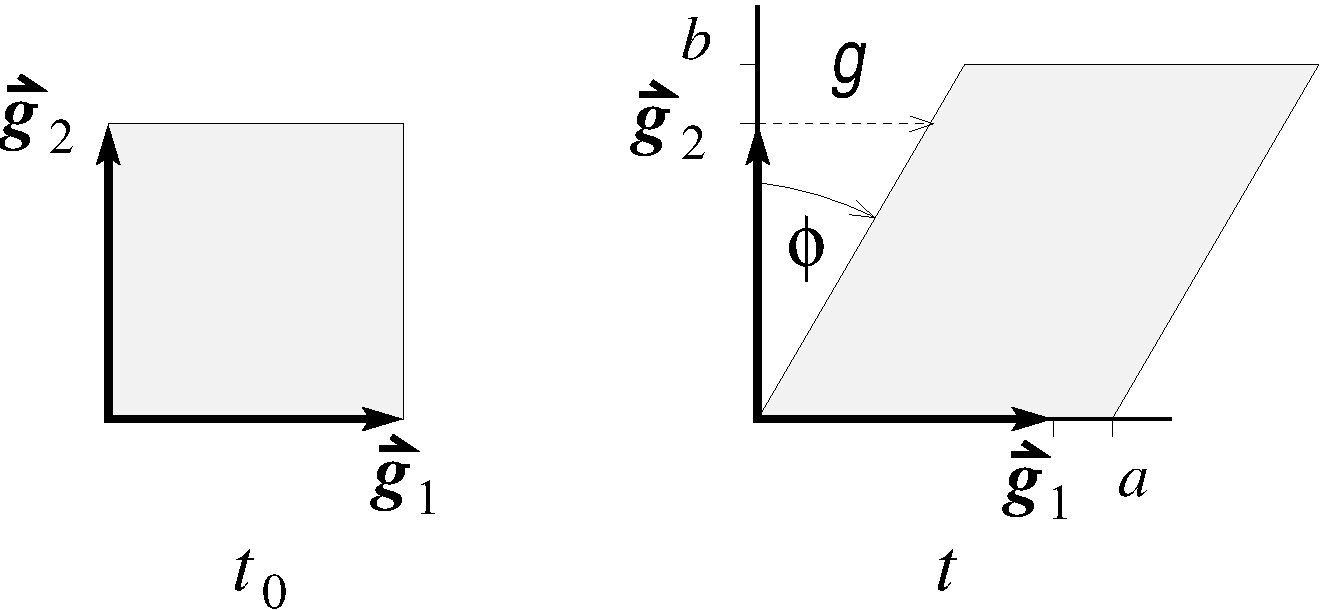
\includegraphics[width=8cm]{figures/deformation.pdf}
	\caption{Physical attributes of a planar deformation: $a$ and $b$ represent elongations, while $g = \tan \phi$ denotes the extent of shear.  They are measured in a physical frame of reference with unit base vectors $( \vec{\mathbfsf{g}}_1 , \vec{\mathbfsf{g}}_2 )$ where $\vec{\mathbfsf{g}}_1$ embeds in the material.}
	\label{figKinematics}
\end{figure}

An orthogonal tensor $\boldsymbol{\mathcal{R}} = \bigl[ \vec{\mathbfsf{g}}_1 \bigm| \vec{\mathbfsf{g}}_2 \bigr] = \delta_{ij} \, \vec{\mathbfsf{g}}_i \otimes \vec{\mathbfsf{e}}_j = \mathcal{R}_{ij} \, \vec{\mathbfsf{e}}_i \otimes \vec{\mathbfsf{e}}_j$ rotates the reference co-ordinate axes $( \vec{\mathbfsf{e}}_1 , \vec{\mathbfsf{e}}_2 )$ into a physical co-ordinate system $( \vec{\mathbfsf{g}}_1 , \vec{\mathbfsf{g}}_2 )$ through an angle $\theta$, which is the fourth physical attribute arising from a \textbf{QR} factorization of $\mathbfsf{F}$.  This angle of rotation describes an orthogonal matrix whereby
\begin{equation}
\boldsymbol{\mathcal{R}} = \begin{bmatrix}
\cos \theta & -\sin \theta \\
\sin \theta & \cos \theta
\end{bmatrix} 
\label{rotation}
\end{equation}  
with
\begin{equation}
\sin \theta = \frac{F_{21}}
{\sqrt{F_{11}^{\,2} + F_{21}^{\,2}}} , \quad
\cos \theta = \frac{F_{11}}
{\sqrt{F_{11}^{\,2} + F_{21}^{\,2}}} 
\quad \therefore \quad
\theta = \tan^{-1} \left( \frac{F_{21}}{F_{11}} \right)
\label{trigFns}
\end{equation}  
where a positive angle $\theta$ corresponds with a counter\-clockwise rotation of physical axes $( \vec{\mathbfsf{g}}_1 , \vec{\mathbfsf{g}}_2 )$ about reference axes $( \vec{\mathbfsf{e}}_1 , \vec{\mathbfsf{e}}_2 )$.


\subsubsection{Dilemma}
\label{secDilemma} 

Until recently, there has been a tacit assumption in prior applications of Gram-Schmidt factorizations of $\mathbfsf{F}$ that the physical base vectors $( \vec{\mathbfsf{g}}_1 , \vec{\mathbfsf{g}}_2 )$ always satisfy a geometric condition whereby the physical 1-direction $\vec{\mathbfsf{g}}_1$ rotates out of the reference 1-direction $\vec{\mathbfsf{e}}_1$, but this need not always be the case.  Physical vector $\vec{\mathbfsf{g}}_1$ could equally likely rotate out of the 2-direction $\vec{\mathbfsf{e}}_2$ of the reference frame.  At issue is not: How the physical base vectors orient in space?  That is managed by Gram's procedure.  Rather, at issue is: How do the physical base vectors index with respect to the reference base vectors?  

To illustrate this concern, consider two deformation histories, as drawn in Fig.~\ref{figDilemma}, each of which describe a simple shear taking place in the plane of a membrane.  In one case shear occurs in the 1-direction, while in the other case shear occurs in the 2-direction.  There are no elongations in this deformation.  These motions lead to Gram-Schmidt factorizations of the deformation gradient, when following the protocol of Eqns.~(\ref{physicalVariables}--\ref{trigFns}), that are described by
\begin{subequations}
	\label{shears}
	\begin{align}
	\mathbfsf{F} = 
	\begin{bmatrix} 1 & \gamma \\ 0 & 1 \end{bmatrix} & \implies 
	\boldsymbol{\mathcal{R}} = 
	\begin{bmatrix} 1 & 0 \\ 0 & 1 \end{bmatrix} , \quad
	\boldsymbol{\mathcal{U}} = 
	\begin{bmatrix} 1 & \gamma \\ 0 & 1  \end{bmatrix} 
	\label{shear1} \\
	\intertext{and}
	\mathbfsf{F} = 
	\begin{bmatrix} 1 & 0 \\ \gamma & 1 \end{bmatrix} & \implies \left\{
	\begin{aligned} \mbox{}
	\boldsymbol{\mathcal{R}} & = \frac{1}{\sqrt{1 + \gamma^2}}
	\begin{bmatrix} 1 & -\gamma \\ \gamma & 1 \end{bmatrix} \\
	\boldsymbol{\mathcal{U}} & = 
	\begin{bmatrix} \sqrt{1 + \gamma^2} & \gamma \\ 
	0 & 1 \bigm/ \sqrt{1 + \gamma^2} \end{bmatrix}
	\end{aligned} \right.
	\label{shear2}
	\end{align}
\end{subequations}
where we see that shear $\mathcal{U}_{12}$ has the same physical interpretation in both cases, viz., $\gamma$, but the elongations $\mathcal{U}_{11}$ and $\mathcal{U}_{22}$ do not, viz., $\mathcal{U}_{11}=1$ and $\mathcal{U}_{22}=1$ in Eq.~(\ref{shear1}), whereas $\mathcal{U}_{11} = \sqrt{1 + \gamma^2}$ and $\mathcal{U}_{22} = 1 / \sqrt{1 + \gamma^2}$ for the motion described in Eq.~(\ref{shear2}).  Consequently, two geometric interpretations are produced for just one physical mode of deformation.  This cannot be!

\begin{figure}
	\centering
	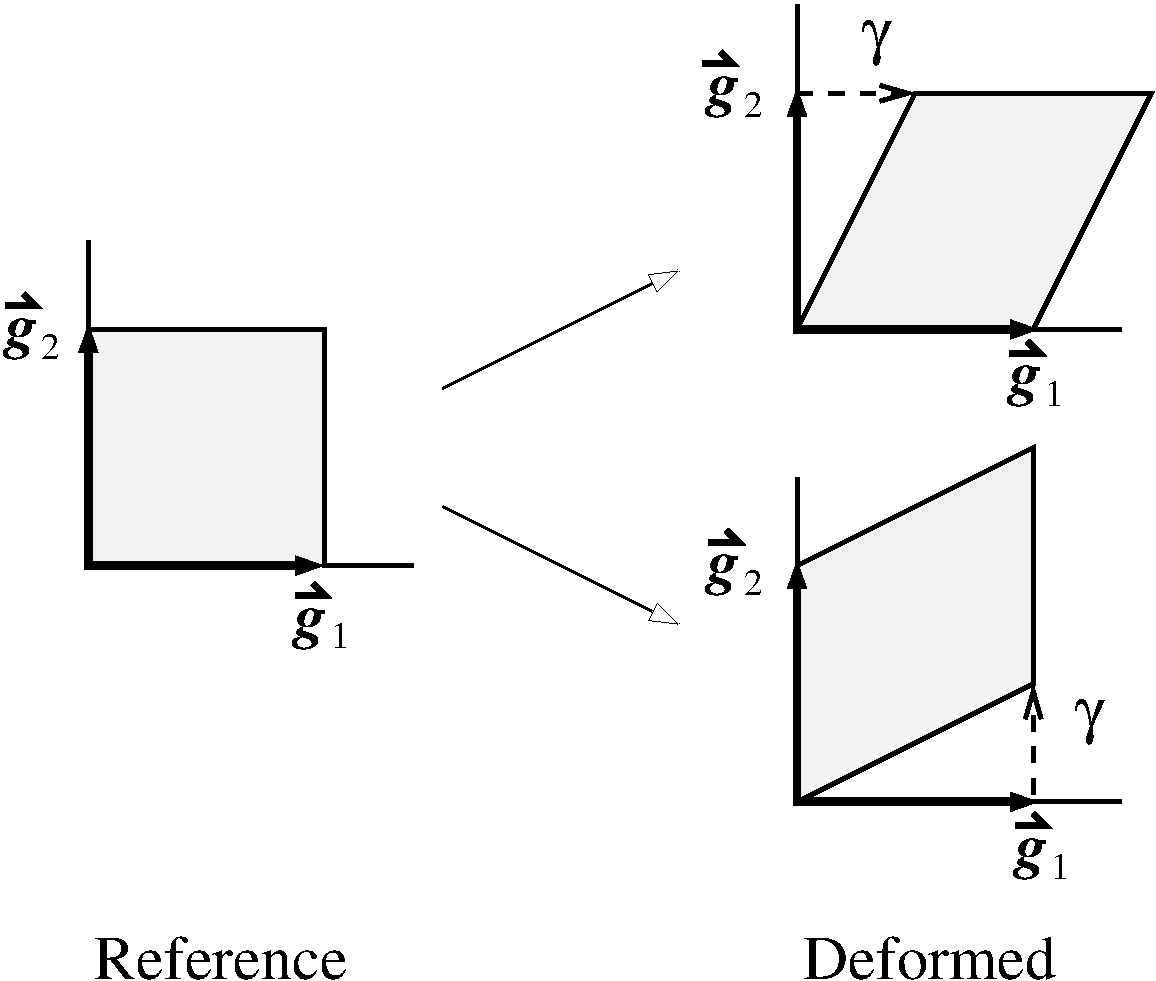
\includegraphics[width=0.5\textwidth]{figures/figDilemma.pdf}
	\caption{The left graphic designates a reference configuration while the right two graphics designate deformed configurations, both in basis $( \vec{\mathbfsf{g}}_1 , \vec{\mathbfsf{g}}_2 )$.  The top graphic associates with the motion of Eqn.~(\ref{shear1}), while the bottom graphic associates with the motion of Eqn.~(\ref{shear2}).}
	\label{figDilemma}
\end{figure}

The only difference between the motions that lead to the two deformation gradients presented in Eq.~(\ref{shears}) is one's choice for labeling the co-ordinate directions.  Matrix operations of row and column pivoting, taken from linear algebra, allow one to transform the lower-triangular form of Eq.~(\ref{shear2}) into an upper-triangular form like Eq.~(\ref{shear1}); hence, producing an unified physical interpretation for both shearing motions, and thereby providing a means for establishing a remedy to this dilemma. 


\subsubsection{Remedy}
\label{secRemedy}

For 2D membranes, there are only two co-ordinate re-indexings that are possible (for 3D solids there are six, cf.\ \S\ref{reindexing3D}).  The default is no re-indexing at all, in which case 
\begin{subequations}
	\label{membraneRelabling}
	\begin{align}
	[ \mathbfsf{P} ] = [ \mathbfsf{P}_0 ] & \defeq 
	\begin{bmatrix} 1 & 0 \\ 0 & 1 \end{bmatrix} & 
	\implies & & \begin{bmatrix}
	\mathcal{F}_{11} & \mathcal{F}_{12} \\
	\mathcal{F}_{21} & \mathcal{F}_{22}
	\end{bmatrix} & \defeq \begin{bmatrix}
	F_{11} & F_{12} \\
	F_{21} & F_{22}
	\end{bmatrix} \label{Q0} \\
	\intertext{while in the second case there is a re-indexing specified by}
	[ \mathbfsf{P} ] = [ \mathbfsf{P}_1 ] & \defeq 
	\begin{bmatrix} 0 & 1 \\ 1 & 0 \end{bmatrix} & 
	\implies & & \begin{bmatrix}
	\mathcal{F}_{11} & \mathcal{F}_{12} \\
	\mathcal{F}_{21} & \mathcal{F}_{22}
	\end{bmatrix} & \defeq \begin{bmatrix}
	F_{22} & F_{21} \\
	F_{12} & F_{11}
	\end{bmatrix}
	\label{Q1}
	\end{align}
\end{subequations}
where components $\mathcal{F}_{ij} = P_{ki} F_{k\ell} P_{\ell j}$ are the components to be used in the Gram-Schmidt factorization presented in \S\ref{secQR2D}, and where $\mathbfsf{P} \in \{ \mathbfsf{P}_0 , \mathbfsf{P}_1 \}$ is orthogonal, i.e., $\mathbfsf{P} \mathbfsf{P}^{\mathsf{T}} = \mathbfsf{P}^{\hspace{-1pt}\mathsf{T}} \mathbfsf{P} = \mathbfsf{I}$ with $\det \mathbfsf{P} = \pm 1$; specifically, $\det \mathbfsf{P}_0 = +1$ while $\det \mathbfsf{P}_1 = -1$.

The challenge in implementing such a strategy is to determine when to switch from $\mathbfsf{P}_0$ (case 1) to $\mathbfsf{P}_1$ (case 2), or back again, viz., from $\mathbfsf{P}_1$ to $\mathbfsf{P}_0$.  Continuity in the physical fields of deformation $(a , b , g )$ must be satisfied in order for such a change in co-ordinate frame to be physically meaningful.  To this end, it is useful to represent the components of a planar deformation gradient as
\begin{equation}
\begin{bmatrix}
\mathcal{F}_{11} & \mathcal{F}_{12} \\
\mathcal{F}_{21} & \mathcal{F}_{22}
\end{bmatrix} =
\begin{cases}
\mathrm{case} \; 1: & \begin{bmatrix}
F_{11} & F_{12} \\
F_{21} & F_{22}
\end{bmatrix}_{\vphantom{|}} = \begin{bmatrix}
x & \beta y \\ \alpha x & y
\end{bmatrix} \\
\mathrm{case} \; 2: & \begin{bmatrix}
F_{22} & F_{21} \\
F_{12} & F_{11}
\end{bmatrix} = \begin{bmatrix}
y & \alpha x \\ \beta y & x
\end{bmatrix}
\end{cases}
\label{deformationGradientRelabelling}
\end{equation}
where $x = F_{11}$ and $y = F_{22}$ are elongations, while ratios $\alpha = F_{21} / F_{11}$ and $\beta = F_{12} / F_{22}$ are magnitudes of shear, as illustrated in Fig.~\ref{figF}.  

\begin{figure}
	\centering
	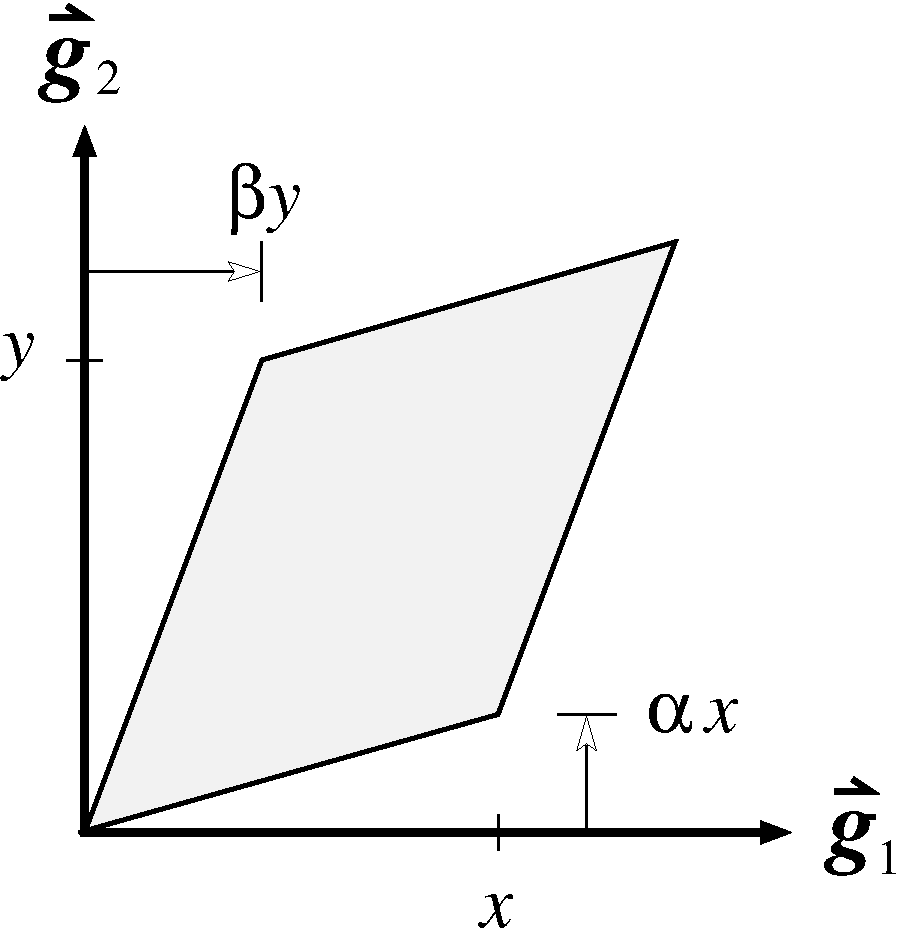
\includegraphics[width=0.3\textwidth]{figures/figF.pdf}
	\caption{A general description for uniform planar deformation, where $x , y \in \mathbb{R}_+$ and $\alpha , \beta \in \mathbb{R}$.  Shears $\alpha$ and $\beta$ are drawn in their positive sense.}
	\label{figF}
\end{figure}

The physical attributes for Laplace stretch, as they pertain to the two cases in Eqn.~(\ref{membraneRelabling}), written in terms of components $F_{ij}$ from $\mathbfsf{F} = F_{ij} \, \vec{\mathbfsf{e}}_i \otimes \vec{\mathbfsf{e}}_j$ as defined in Eqn.~(\ref{deformationGradientRelabelling}), are respectively given by
\begin{subequations}
	\label{physicalAttributes}
	\begin{align}
	\tilde{a} & = x \sqrt{1 + \alpha^2} & 
	\hat{a} & = y \sqrt{1 + \beta^2} 
	\label{aAttribute} \\
	\tilde{b} & = y ( 1 - \alpha \beta ) \bigm/ \sqrt{1 + \alpha^2} &
	\hat{b} & = x ( 1 - \alpha \beta ) \bigm/ \sqrt{1 + \beta^2} 
	\label{bAttribute} \\ 
	\tilde{g} & = y ( \alpha + \beta ) \bigm/ x (1 + \alpha^2) &
	\hat{g} & = x ( \alpha + \beta ) \bigm/ y (1 + \beta^2)
	\label{gAttribute} \\
	\tilde{\theta} & = \tan^{-1} ( -\alpha ) & 
	\hat{\theta} & = \tan^{-1} ( -\beta )
	\label{thetaAttribute}
	\end{align}
\end{subequations}
where attributes in the left column apply to case~1 (i.e., Eqn.~\ref{Q0}) while those in the right column apply to case~2 (viz., Eqn.~\ref{Q1}).  The actual set of physical attributes $\{ a, b, g, \theta \}$ that are to be used when quantifying Laplace stretch and its inverse, according to Eqn.~(\ref{LaplaceStretch}), are then selected via the strategy  
\begin{subequations}
	\label{attributeMaps}
	\begin{align}
	\mathrm{if} \; | \tilde{g} | \geq | \hat{g} | : & &
	\{ \tilde{a} , \tilde{b} , \tilde{g} , \tilde{\theta} \} &
	\mapsto \{ a , b , g , \theta \}  \\
	\mathrm{else} \; | \tilde{g} | \leq | \hat{g} | : & &
	\{ \hat{a} , \hat{b} , \hat{g} , \hat{\theta} \} & 
	\mapsto \{ a , b , g , \theta \}
	\end{align}
\end{subequations}
where it is easily verified that $\tilde{a} = \hat{a}$ and $\tilde{b} = \hat{b}$ whenever $\tilde{g} = \hat{g}$; consequently, the physical attributes of deformation $a , b , g$ remain continuous across a co-ordinate switch, however, the angle of co-ordinate rotation $\theta$ will not be continuous across such a switch between co-ordinate frames, as they represent rotations out of different co-ordinate directions.

The above strategy returns matrices for the rotation and Laplace stretch described in Eqn.~(\ref{shear1}) for both deformation gradients presented in Eqn.~(\ref{shears}). The dilemma is remedied.  Laplace stretch, as remedied, therefore has an unique physical interpretation.  

This above process is the 2D version of the 3D version presented earlier in \S\ref{reindexing3D}.  It is easier to understand what is happening in the 2D case, which is why more detail is presented here.  It may certainly happen that even when the 3D co-ordinates are re-indexed there may be one or more of the pentagons whose 2D co-ordinates need to be re-indexed, too.

There are three kinematic variables that describe deformation in a planar membrane: elongation ratios $a$ and $b$ and simple shear $g$.  These variables will vary both temporally and spatially whenever Wachspress' shape functions are used, as described above.  The fields introduced above are exported from module \texttt{membranes} outlined in \ref{appMembranes}.

\subsection{Thermodynamic Strains and Strain Rates}

In terms of the above physical attributes for stretch, i.e., $a$, $b$ and $g$, and their reference values, viz., $a_0$, $b_0$ and $g_0$, one can define a set of strain attributes derived from thermo\-dynamics, specifically \cite{Freed17}
\begin{subequations}
    \label{thermodynamicStrains2D}
    \begin{align}
    \xi & \defeq \ln \left( \sqrt{\frac{a}{a_0} \frac{b}{b_0}} \right) & 
    \mathrm{d} \xi & = \frac{1}{2} \left( \frac{\mathrm{d}a}{a} + 
    \frac{\mathrm{d}b}{b} \right) \\
    \varepsilon & \defeq \ln \left( \sqrt{\frac{a}{a_0} \frac{b_0}{b}} \right) &
    \mathrm{d} \varepsilon & = \frac{1}{2} \left( \frac{\mathrm{d}a}{a} - 
    \frac{\mathrm{d}b}{b} \right) \\
    \gamma & \defeq g - g_0 & 
    \mathrm{d} \gamma & = \mathrm{d} g
    \end{align}
\end{subequations}
whose rates are exact differentials, i.e., they are independent of path---a tacit requirement from thermo\-dynamics \cite{Caratheodory09}.  Here $\xi$ denotes dilation, $\varepsilon$ denotes squeeze, and $\gamma$ denotes shear. 

\subsubsection{Stretch Rates}

The following approximations for stretch rates were derived by Freed \&\ Zamani \cite{FreedZamani18}.  From these, the various strain rates listed in Eqn.~(\ref{thermodynamicStrains2D}) can be established.  

A forward difference formula is used to approximate rates in the reference configuration for the various stretch attributes, as obtained from $\dot{\boldsymbol{\mathcal{U}}}_0 = ( \boldsymbol{\mathcal{U}}_1 -  \boldsymbol{\mathcal{U}}_0 ) / h + \mathcal{O}(h)$.  This produces
\begin{equation}
\mathrm{d} a_0 = \frac {a_1 - a_0}{h} , \quad 
\mathrm{d} b_0 = \frac {b_1 - b_0}{h} , \quad 
\mathrm{d} g_0 = \frac{a_1}{a_0} 
\left( \frac{g_1 - g_0}{h} \right) .
\label{forwardDifference1stOrder2D}
\end{equation}
A backward difference formula $\dot{\boldsymbol{\mathcal{U}}}_1 = ( \boldsymbol{\mathcal{U}}_1 - \boldsymbol{\mathcal{U}}_0 ) / h + \mathcal{O}(h)$ is used to estimate rates for the various stretch attributes at the end of its first integration step, from which it follows that
\begin{equation}
\mathrm{d} a_1 = \frac {a_1 - a_0}{h} , \quad
\mathrm{d} b_1 = \frac {b_1 - b_0}{h} , \quad
\mathrm{d} g_1 = \frac{a_0}{a_1} 
\left(\frac{g_1 - g_0}{h} \right) .
\label{backwardDifference1stOrder2D}
\end{equation}
Curiously, there is a distinction in how the shear rates are approximated at the two nodes for this first interval of integration.

Equations (\ref{forwardDifference1stOrder2D} \& \ref{backwardDifference1stOrder2D}) are first-order approximations for these derivatives.  Second-order approximations can be established whenever $n > 0$ provided the stepsize for step $[n, n+1]$ equals the stepsize for step $[n-1, n]$, where state $n=0$ associates with an initial condition.  The backward difference formula  $\dot{\boldsymbol{\mathcal{U}}}_{n+1} = ( 3 \, \boldsymbol{\mathcal{U}}_{n+1} -  4 \, \boldsymbol{\mathcal{U}}_{n} + \boldsymbol{\mathcal{U}}_{n-1} ) / 2h + \mathcal{O}(h^2)$ then produces stretch rates of
\begin{equation}
\begin{aligned}
\mathrm{d} a_{n+1} & 
= \frac {3a_{n+1} - 4a_{n} +  a_{n-1}}{2h} \\ 
\mathrm{d} b_{n+1} & 
= \frac {3b_{n+1} - 4b_{n} +  b_{n-1}}{2h} \\
\mathrm{d} g_{n+1} & 
= \frac{2a_{n}} {a_{n+1}} \left(\frac{g_{n+1} - g_{n}}{h} \right) - \frac{a_{n-1}}{a_{n+1}} \left( \frac{g_{n+1} - g_{n-1}}{2h} \right) 
\end{aligned}
\label{backwardDifference2ndOrder2D}
\end{equation}
which will require $a_{n-1}$, $b_{n-1}$ and $g_{n-1}$ to be stored in a finite element setting.

\section{3D Irregular Dodecahedra}

The primary kinematic variables needed to describe the deformation of an irregular dodecahedron used as a model for an alveolar sac are its volume $V$ (see \S\ref{sec:geometries}) and the differential change in volume $\mathrm{d}V$, with the former following from Eq.~(\ref{tetrahedralVolume}) and the latter coming from a suitable finite difference formula.  Whenever the material filling an alveolar sac is air (its normal healthy condition), no further breakdown of these kinematics is required.  

However, whenever an alveolar sac is filled with fluid (blood, interstitial fluids, pflem, etc.) this fluid can be expected to behave solid-like in the face of a passing shock wave.  In this situation, non-uniform measures for strain (i.e., shears) can be expected to arise.

\subsection{Shape Functions for Interpolating an Irregular Tetrahedron}

The shape functions associated with the four vertices of a tetrahedron $N_i$, $i = 1, 2, 3, 4,$ that are used in this work are defined as follows
\begin{subequations}
    \begin{align}
    N_1 & = 1 - \xi - \eta - \zeta , \quad
    N_2 = \xi , \quad
    N_3 = \eta , \quad
    N_4 = \zeta \\
    \intertext{where $\xi$, $\eta$ and $\zeta$ represent its natural co-ordinates whereby $0 \leq \xi \leq 1$, $0 \leq \eta \leq 1-\xi$ and $0 \leq \zeta \leq 1-\xi-\eta$.  Gradients of these shape functions are} 
    N_{1,\xi} & = -1 , \quad N_{1,\eta} = -1 , \quad N_{1,\zeta} = -1 \notag \\
    N_{2,\xi} & = 1 , \quad \phantom{-} N_{2,\eta} = 0 , \quad \phantom{-} N_{2,\zeta} = 0 \notag \\
    N_{3,\xi} & = 0 , \quad \phantom{-} N_{3,\eta} = 1 , \quad \phantom{-} N_{3,\zeta} = 0 \notag \\
    N_{4,\xi} & = 0 , \quad \phantom{-} N_{4,\eta} = 0 , \quad \phantom{-} N_{4,\zeta} = 1 
    \end{align}
\end{subequations}
and consequently the deformation gradient will be constant throughout its volume.

\subsubsection{Deformation Gradient for an Irregular Tetrahedron}

The deformation gradient for a volume element is constructed from
\begin{equation}
    \mathbfsf{F} ( \xi , \eta , \zeta ) = \begin{bmatrix} 1 & 0 & 0 \\
    0 & 1 & 0 \\ 0 & 0 & 1 \end{bmatrix} + \begin{bmatrix}
    \partial u / \partial \xi & \partial u / \partial \eta & \partial u / \partial \zeta \\
    \partial v / \partial \xi & \partial v / \partial \eta & \partial v / \partial \zeta \\
    \partial w / \partial \xi & \partial w / \partial \eta & \partial w / \partial \zeta
    \end{bmatrix} \begin{bmatrix}
    \partial x_0 / \partial \xi & \partial x_0 / \partial \eta & \partial x_0 / \partial \zeta \\
    \partial y_0 / \partial \xi & \partial y_0 / \partial \eta & \partial y_0 / \partial \zeta \\
    \partial z_0 / \partial \xi & \partial z_0 / \partial \eta & \partial z_0 / \partial \zeta
    \end{bmatrix}^{-1}
\end{equation}
such that, for the four-node tetrahedron considered here, one has
\begin{subequations}
    \begin{align}
    \begin{bmatrix}
    \partial u / \partial \xi & \partial u / \partial \eta & \partial u / \partial \zeta \\
    \partial v / \partial \xi & \partial v / \partial \eta & \partial v / \partial \zeta \\
    \partial w / \partial \xi & \partial w / \partial \eta & \partial w / \partial \zeta
    \end{bmatrix} & = \begin{bmatrix}
    \sum_{i=1}^4 N_{i,\xi} u_i & \sum_{i=1}^4 N_{i,\eta} u_i & \sum_{i=1}^4 N_{i,\zeta} u_i \\
    \sum_{i=1}^4 N_{i,\xi} v_i & \sum_{i=1}^4 N_{i,\eta} v_i & \sum_{i=1}^4 N_{i,\zeta} v_i \\
    \sum_{i=1}^4 N_{i,\xi} w_i & \sum_{i=1}^4 N_{i,\eta} w_i & \sum_{i=1}^4 N_{i,\zeta} w_i 
    \end{bmatrix} \notag \\
    & = \begin{bmatrix}
    u_2 - u_1 & u_3 - u_1 & u_4 - u_1 \\
    v_2 - v_1 & v_3 - v_1 & v_4 - v_1 \\
    w_2 - w_1 & w_3 - w_1 & w_4 - w_1
    \end{bmatrix} \\
    \intertext{whose nodal displacements $\mathbfit{u}_i \defeq \mathbfit{x}_i - \mathbfit{x}_{0i}$, $i=1,2,3,4$, have components $\mathbfit{u}_i = u_i \, \vec{\mathbfsf{E}}_1 + v_i \, \vec{\mathbfsf{E}}_2 + w_i \, \vec{\mathbfsf{E}}_3$ when evaluated in the co-ordinate frame of a dodecahedron $( \vec{\mathbfsf{E}}_1 , \vec{\mathbfsf{E}}_2 , \vec{\mathbfsf{E}}_3 )$ with $u_i \defeq x_i - x_{0i}$, $v_i \defeq y_i - y_{0i}$ and $w_i \defeq z_i - z_{0i}$, and where}
    \begin{bmatrix}
    \partial x_0 / \partial \xi & \partial x_0 / \partial \eta & \partial x_0 / \partial \zeta \\
    \partial y_0 / \partial \xi & \partial y_0 / \partial \eta & \partial y_0 / \partial \zeta \\
    \partial z_0 / \partial \xi & \partial z_0 / \partial \eta & \partial z_0 / \partial \zeta
    \end{bmatrix} & = \begin{bmatrix}
    \sum_{i=1}^4 N_{i,\xi} x_{0i} & \sum_{i=1}^4 N_{i,\eta} x_{0i} & \sum_{i=1}^4 N_{i,\zeta} x_{0i} \\
    \sum_{i=1}^4 N_{i,\xi} y_{0i} & \sum_{i=1}^4 N_{i,\eta} y_{0i} & \sum_{i=1}^4 N_{i,\zeta} y_{0i} \\
    \sum_{i=1}^4 N_{i,\xi} z_{0i} & \sum_{i=1}^4 N_{i,\eta} z_{0i} & \sum_{i=1}^4 N_{i,\zeta} z_{0i}
    \end{bmatrix} \notag \\
    & = \begin{bmatrix}
    x_{02} - x_{01} & x_{03} - x_{01} & x_{04} - x_{01} \\
    y_{02} - y_{01} & y_{03} - y_{01} & y_{04} - y_{01} \\
    z_{02} - z_{01} & z_{03} - z_{01} & z_{04} - z_{01}
    \end{bmatrix} \\
    \intertext{whose initial nodal positions are $\mathbfit{x}_{0i} = x_{0i} \, \vec{\mathbfsf{E}}_1 + y_{0i} \, \vec{\mathbfsf{E}}_2 + z_{0i} \, \vec{\mathbfsf{E}}_3$.  This matrix is invertible, becuase the four vertices of the tetrahedron are distinct.  The Jacobian matrix is given by}
    \mathbf{J} \defeq \begin{bmatrix}
    \partial x / \partial \xi & \partial x / \partial \eta & \partial x / \partial \zeta \\
    \partial y / \partial \xi & \partial y / \partial \eta & \partial y / \partial \zeta \\
    \partial z / \partial \xi & \partial z / \partial \eta & \partial z / \partial \zeta
    \end{bmatrix} & = \begin{bmatrix}
    \sum_{i=1}^4 N_{i,\xi} x_{i} & \sum_{i=1}^4 N_{i,\eta} x_{i} & \sum_{i=1}^4 N_{i,\zeta} x_{i} \\
    \sum_{i=1}^4 N_{i,\xi} y_{i} & \sum_{i=1}^4 N_{i,\eta} y_{i} & \sum_{i=1}^4 N_{i,\zeta} y_{i} \\
    \sum_{i=1}^4 N_{i,\xi} z_{i} & \sum_{i=1}^4 N_{i,\eta} z_{i} & \sum_{i=1}^4 N_{i,\zeta} z_{i}
    \end{bmatrix} \notag \\
    & = \begin{bmatrix}
    x_{2} - x_{1} & x_{3} - x_{1} & x_{4} - x_{1} \\
    y_{2} - y_{1} & y_{3} - y_{1} & y_{4} - y_{1} \\
    z_{2} - z_{1} & z_{3} - z_{1} & z_{4} - z_{1}
    \end{bmatrix}
    \end{align}
\end{subequations}
which is used in integrations.  Its current nodal positions are $\mathbfit{x}_{i} = x_i \, \vec{\mathbfsf{E}}_1 + y_i \, \vec{\mathbfsf{E}}_2 + z_i \, \vec{\mathbfsf{E}}_3$, $i=1,2,3,4$.  The Jacobian matrix is also invertible, because the four vertices of a tetrahedron are distinct.

\subsection{\textbf{QR} Factorization of $\mathbfsf{F}$}
\label{secQR3D}

The re-indexed deformation gradient presented in \S\ref{reindexing3D} has a Gram-Schmidt decomposition that we denote as $\mathbfsf{F} = \boldsymbol{\mathcal{RU}}$ wherein $\boldsymbol{\mathcal{R}} = \bigl[ \vec{\mathbfsf{g}}_1 \bigm| \vec{\mathbfsf{g}}_2 \bigm| \vec{\mathbfsf{g}}_3 \bigr] = \delta_{ij} \, \vec{\mathbfsf{g}}_i \otimes \vec{\mathbfsf{E}}_j = \mathcal{R}_{ij} \, \vec{\mathbfsf{E}}_i \otimes \vec{\mathbfsf{E}}_j$ is a Gram rotation with orthogonal components, and $\boldsymbol{\mathcal{U}} = \mathcal{U}_{ij} \, \vec{\mathbfsf{E}}_i \otimes \vec{\mathbfsf{E}}_j$ is a Laplace stretch \cite{Freedetal19} with upper-triangular components, so that $\mathbfsf{F} = \mathcal{F}_{ij} \, \vec{\mathbfsf{E}}_i \otimes \vec{\mathbfsf{E}}_j = \mathcal{R}_{ik\,} \mathcal{U}_{kj} \, \vec{\mathbfsf{E}}_i \otimes \vec{\mathbfsf{E}}_j$.

The components of Laplace stretch $\mathcal{U}_{ij}$ are readily gotten through a Cholesky factorization of the right Cauchy-Green deformation tensor, here taken to be $\mathbfsf{C} = \mathcal{C}_{ij} \, \vec{\mathbfsf{E}}_i \otimes \vec{\mathbfsf{E}}_j$ with components $\mathcal{C}_{ij} = \mathcal{F}_{ki\,} \mathcal{F}_{kj}$ (no eigen analysis is required).  Laplace stretch has elements \cite{Freed17}
\begin{equation} 
\boldsymbol{\mathcal{U}} = 
\begin{bmatrix}
a & a \gamma & a \beta \\ 0 & b & b \alpha \\ 0 & 0 & c
\end{bmatrix} 
\quad \text{with inverse} \quad
\boldsymbol{\mathcal{U}}^{-1} = \begin{bmatrix}
1/a & -\gamma / b & -( \beta - \alpha\gamma ) / c \\
0 & 1/b & -\alpha / c \\
0 & 0 & 1/c
\end{bmatrix}
\label{LaplaceStretch3D}
\end{equation}
with components $\mathcal{U}_{ij}$ being evaluated according to the formul\ae\ \cite{Srinivasa12}
\begin{equation}
\begin{aligned}
\mathcal{U}_{11} & = \sqrt{\mathcal{C}_{11}} & 
\mathcal{U}_{12} & = \mathcal{C}_{12} / \mathcal{U}_{11} &
\mathcal{U}_{13} & = \mathcal{C}_{13} / \mathcal{U}_{11} \\
\mathcal{U}_{21} & = 0 &
\mathcal{U}_{22} & = \sqrt{\mathcal{C}_{22} - \mathcal{U}_{12}^{\,2}} &
\mathcal{U}_{23} & = \bigl( \mathcal{C}_{23} - 
\mathcal{U}_{12\,} \mathcal{U}_{13} \bigr) / \mathcal{U}_{22} \\
\mathcal{U}_{31} & = 0 &
\mathcal{U}_{32} & = 0 & 
\mathcal{U}_{33} & = \sqrt{\mathcal{C}_{33} - \mathcal{U}_{13}^{\,2} - 
    \mathcal{U}_{23}^{\,2}}
\end{aligned}
\label{LagrangianLaplaceStretch3D}
\end{equation}
so that
\begin{equation}
a \defeq \mathcal{U}_{11} , \quad
b \defeq \mathcal{U}_{22} , \quad
c \defeq \mathcal{U}_{33} , \quad
\alpha \defeq \frac{\mathcal{U}_{23}}{\mathcal{U}_{22}} , \quad
\beta \defeq \frac{\mathcal{U}_{13}}{\mathcal{U}_{11}} , \quad
\gamma \defeq \frac{\mathcal{U}_{12}}{\mathcal{U}_{11}}
\label{LagrangianPhysicalAttributes3D}
\end{equation}
where $a$, $b$ and $c$ are three, orthogonal, elongation ratios, and where $\alpha$, $\beta$ and $\gamma$ are three, orthogonal, simple shears, with $a_0$, $b_0$, $c_0$, $\alpha_0$, $\beta_0$ and $\gamma_0$ denoting their values in some reference state. The elongations must be positive whereas the shears may be of either sign. Collectively, they constitute a complete set of physical attributes for describing stretch from which constitutive equations can then be constructed.

\subsection{Thermodynamic Strains and Strain Rates}

In terms of the above physical attributes for stretch, one can define a set of strain attributes derived from thermo\-dynamics, specifically \cite{Freed17}
\begin{subequations}
    \label{thermodynamicStrains3D}
    \begin{align}
    \Xi & \defeq \ln \left( \sqrt[3]{\frac{a}{a_0} \frac{b}{b_0} \frac{c}{c_0}} \right) & 
    \mathrm{d} \Xi & = \frac{1}{2} \left( \frac{\mathrm{d}a}{a} + 
    \frac{\mathrm{d}b}{b} + \frac{\mathrm{d}c}{c} \right) \\
    \varepsilon_1 & \defeq \ln \left( \sqrt[3]{\frac{a}{a_0} \frac{b_0}{b}} \right) &
    \mathrm{d} \varepsilon_1 & = \frac{1}{3} \left( \frac{\mathrm{d}a}{a} - 
    \frac{\mathrm{d}b}{b} \right) \\
    \varepsilon_2 & \defeq \ln \left( \sqrt[3]{\frac{b}{b_0} \frac{c_0}{c}} \right) &
    \mathrm{d} \varepsilon_2 & = \frac{1}{3} \left( \frac{\mathrm{d}b}{b} - 
    \frac{\mathrm{d}c}{c} \right) \\
    \gamma_1 & \defeq \alpha - \alpha_0 & 
    \mathrm{d} \gamma_1 & = \mathrm{d} \alpha \\
    \gamma_2 & \defeq \beta - \beta_0 & 
    \mathrm{d} \gamma_2 & = \mathrm{d} \beta \\
    \gamma_3 & \defeq \gamma - \gamma_0 & 
    \mathrm{d} \gamma_3 & = \mathrm{d} \gamma
    \end{align}
\end{subequations}
whose rates are exact differentials, i.e., they are independent of path---a tacit requirement from thermo\-dynamics \cite{Caratheodory09}.  Here $\Xi$ represents dilatation, $\varepsilon_1$ is a squeeze in the 12~plane, and $\varepsilon_2$ is a squeeze in the 23-plane, while $\gamma_1$ is a shear in the 23~plane, $\gamma_2$ is a shear in the 13~plane, and $\gamma_3$ is a shear in the 12~plane, which are three, orthogonal, simple shearing motions.  There is a third squeeze, too, viz., $\varepsilon_3 = -\varepsilon_1 - \varepsilon_2$, but it is not an independent descriptor of strain.

\subsubsection{Stretch Rates}

The following approximations for stretch rates were derived by Freed \&\ Zamani \cite{FreedZamani18}.  From these, the various strain rates listed in Eqn.~(\ref{thermodynamicStrains3D}) can be established.  

A forward difference formula is used to approximate rates in the reference configuration for the various stretch attributes, as obtained from $\dot{\boldsymbol{\mathcal{U}}}_0 = ( \boldsymbol{\mathcal{U}}_1 -  \boldsymbol{\mathcal{U}}_0 ) / h + \mathcal{O}(h)$.  This produces
\begin{equation}
\begin{aligned}
\mathrm{d} a_0 &
= \frac {a_1 - a_0}{h} \quad &
\mathrm{d} \alpha_0 & 
= \frac{b_1}{b_0} \left(\frac{\alpha_1 - \alpha_0}{h} \right) \\
\mathrm{d} b_0 & 
= \frac {b_1 - b_0}{h} \quad & 
\mathrm{d} \beta_0 & 
= \frac{a_1}{a_0} \left( \frac{\beta_1 - \beta_0}{h} \right) \\
\mathrm{d} c_0 & 
= \frac {c_1 - c_0}{h} \quad & 
\mathrm{d} \gamma_0 & \approx \frac{a_1}{a_0} \left( \frac{\gamma_1 - \gamma_0}{h}\right) .
\end{aligned}
\label{forwardDifference1stOrder3D}
\end{equation}
A backward difference formula $\dot{\boldsymbol{\mathcal{U}}}_1 = ( \boldsymbol{\mathcal{U}}_1 -  \boldsymbol{\mathcal{U}}_0 ) / h + \mathcal{O}(h)$ is used to estimate rates for the various stretch attributes at the end of its first integration step, from which it follows that
\begin{equation}
\begin{aligned}
\mathrm{d} a_1 & 
= \frac {a_1 - a_0}{h} \;\; & 
\mathrm{d} \alpha_1 & 
= \frac {b_0}{b_1} \left( \frac{\alpha_1 - \alpha_0}{h} \right) \\
\mathrm{d} b_1 & 
= \frac {b_1 - b_0}{h} \;\; & 
\mathrm{d} \beta_1 & 
= \frac {a_0} {a_1} \left( \frac{\beta_1 - \beta_0}{h} \right) \\
\mathrm{d} c_1 & 
= \frac {c_1 - c_0}{h} \;\; & 
\mathrm{d} \gamma_1 & 
= \frac{a_0}{a_1} \left(\frac{\gamma_1 - \gamma_0}{h} \right) .
\end{aligned}
\label{backwardDifference1stOrder3D}
\end{equation}
Curiously, there is a distinction in how the shear rates are approximated at the two nodes for this first interval of integration.

Equations (\ref{forwardDifference1stOrder3D} \& \ref{backwardDifference1stOrder3D}) are first-order approximations for these derivatives.  Second-order approximations can be established whenever $n > 0$ provided the stepsize for step $[n, n+1]$ equals the stepsize for step $[n-1, n]$, where state $n=0$ associates with an initial condition.  The backward difference formula  $\dot{\boldsymbol{\mathcal{U}}}_{n+1} = ( 3 \, \boldsymbol{\mathcal{U}}_{n+1} -  4 \, \boldsymbol{\mathcal{U}}_{n} + \boldsymbol{\mathcal{U}}_{n-1} ) / 2h + \mathcal{O}(h^2)$ produces differential stretch rates of
\begin{equation}
\begin{aligned}
\mathrm{d} a_{n+1} & 
= \frac {3a_{n+1} - 4a_{n} +  a_{n-1}}{2h} \\ 
\mathrm{d} b_{n+1} & 
= \frac {3b_{n+1} - 4b_{n} +  b_{n-1}}{2h} \\
\mathrm{d} c_{n+1} & 
= \frac {3c_{n+1} - 4c_{n} +  c_{n-1}}{2h} \\
\mathrm{d} \alpha_{n+1} & 
= \frac{2b_{n}} {b_{n+1}} \left( \frac{\alpha_{n+1} - \alpha_{n}}{h} \right) - \frac{b_{n-1}} {b_{n+1}} \left( \frac{\alpha_{n+1} - \alpha_{n-1}}{2h} \right) \\
\mathrm{d} \beta_{n+1} & 
= \frac{2a_{n}}{a_{n+1}} \left( \frac{\beta_{n+1} - \beta_{n} }{h} \right) - \frac{a_{n-1}} {a_{n+1}} \left( \frac{\beta_{n+1} - \beta_{n-1}}{2h} \right) \\ 
\mathrm{d} \gamma_{n+1} & 
= \frac{2a_{n}} {a_{n+1}} \left(\frac{\gamma_{n+1} - \gamma_{n}}{h} \right) - \frac{a_{n-1}}{a_{n+1}} \left( \frac{\gamma_{n+1} - \gamma_{n-1}}{2h} \right) 
\end{aligned}
\label{backwardDifference2ndOrder3D}
\end{equation}
which require data to be stored for the previous state associated with step $n-1$.

\section{Code Verification: Kinematics}
\label{sec:verification}

The thermodynamic conjugate pairs of Freed \textit{et~al}.\ \cite{Freed17,Freedetal17,FreedZamani19} result in the following geometric/thermo\-dynamic strain measures for our dodecahedral model: for 1D rods, an axial strain $e = \ln ( L / L_0 )$; for 2D membranes, a dilation $\xi = \ln \sqrt{ab/a_0b_0} = \ln \sqrt{A/A_0}$, a squeeze (or pure shear) $\varepsilon = \ln \sqrt{ab_0/a_0b} = \ln \sqrt{\Gamma / \Gamma_0}$, and a (simple) shear $\gamma = g - g_0$; and for 3D dodecahedra, a dilatation $\Xi = \ln \sqrt[3]{V \! / V_0}$ and, for those cases where the medium within an alveolar sac can support non-uniform stresses, two squeezes $\varepsilon_1 = \ln \sqrt[3]{a b_0 / a_0 b}$ and $\varepsilon_2 = \ln \sqrt[3]{b c_0 / b_0 c}$ plus three shears $\gamma_1 = \alpha - \alpha_0$, $\gamma_2 = \beta - \beta_0$ and $\gamma_3 = \gamma - \gamma_0$. 

\subsection{Isotropic Motions}

Imposing the uniform far-field motion of a volumetric expansion onto our dodecahedral model results in a dodecahedral dilatation ($\Xi \defeq \ln \sqrt[3]{ V \! / V_0 }$) that equals its pentagonal dilation ($\xi \defeq \ln \sqrt{ A / A_0 }$) that equals its chordal strain ($e \defeq \ln ( L / L_0 )$).  These three strain measures follow from the 3-mode thermo\-dynamic theory of Freed \textit{et~al}.\ \cite{Freedetal17,FreedZamani19}.  Other choices for strain measures do not result in one-to-one relationships when exposed to an isotropic motion like those observed here.  This is a particularly useful result in that it establishes a meaningful scaling in terms of strains between the three dimensions, cf.\ Fig.~\ref{figDilatation}.  It also provides for a verification of the numerical implementation of our dodecahedral model.  

\begin{figure}
	\centering
	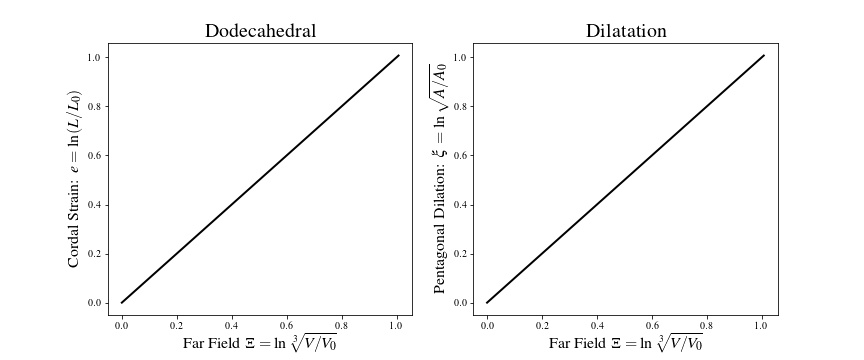
\includegraphics[width=0.9\textwidth]{figures/dilatation.jpg}
	\caption{Response of a dodecahedron exposed to an isotropic motion of dilatation.  The abscissa is the control variable and the ordinates are response variables. The right graphic plots the areal response of the pentagons $\xi = \ln \sqrt{A / A_0}$, while the left graphic plots the axial response of the chords $e = \ln ( L / L_0)$. Both are plotted against the volumetric response of the dodecahedron $\Xi = \ln \sqrt[3]{V \! / V_0}$.  Here $V$ denotes dodecahedral volume, $A$ denotes pentagonal area, and $L$ denotes chordal length, all being evaluated in the current state, whose reference values are $V_0$, $A_0$ and $L_0$.}
	\label{figDilatation}
\end{figure}

\subsubsection{Geometric vs.\ Thermodynamic Strains}

There are two types of strain measures that one can use to quantify deformation within a pentagon of a dodecahedron: geometric and thermo\-dynamic.  For the uniform far-field motion of volumetric expansion, only the thermo\-dynamic strain known as dilation, i.e., $\xi = \ln \sqrt{ab/a_0b_0}$, varies with the motion, and its response equals that of the geometric strain $\ln \sqrt{A / A_0}$, see Fig.~\ref{figDilatation2}.  Also present in this graph is an observation that the thermo\-dynamic strains for squeeze $\varepsilon$ and shear $\gamma$ do not contribute under motions of pure dilatation, as expected.  This further verifies the numerical implementation of our dodecahedral model.

\begin{figure}
	\centering
	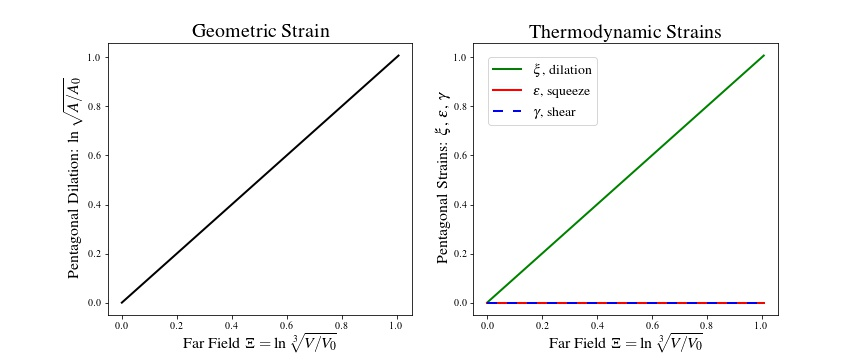
\includegraphics[width=0.9\textwidth]{figures/dilatationGeoVsThermo.jpg}
	\caption{Response of a dodecahedron exposed to a far-field isotropic motion of dilatation.  The abscissa is the control variable and the ordinates are response variables. The right graphic plots the three thermo\-dynamic strains, as they apply to a pentagon, while the left graphic plots the geometric strain of a pentagon.}
	\label{figDilatation2}
\end{figure}

To put this into perspective, we compare with studies done by multiple investigators where ratios of alveolar surface area, viz., $A/A_0$, have been measured in rat, rabbit, guinea pig, and cat, cf.\ Roan \& Waters \cite[Table~1]{RoanWaters11}.  These experiments considered ranges that went as low as 25\% and as high as 100\% of total lung capacity.  Taking statistics of their tabulation produced results of: $A/A_0 = 1.47 \pm 0.44$ during inflation and $A/A_0 = 1.18 \pm 0.14$ during deflation, which correspond to a $\xi = \ln\sqrt{A/A_0} = 0.19 \pm 0.18$ for inflation and a $\xi = \ln\sqrt{A/A_0} = 0.08 \pm 0.07$ for deflation.  These areal strains values coincide with the chordal strains of $e=\ln(L/L_0) = 0.13$ measured in~vivo around the periphery of an alveolus in rat lung, as reported by Perlman \& Bhattachary \cite{PerlmanBhattacharya07}.  Our kinematics have been verified well past these physiologic ranges, viz., for dilatations up to 100\% logarithmic strain. 

\subsection{Isochoric Motions}

The motions of pure and simple shears are volume preserving.  Imposing these shears as far-field motions onto our dodecahedral model produced the results displayed in Fig.~\ref{figIsochoric}.  For a simple shear, the numerical model is in error by about machine precision, i.e., $\epsilon_m \approx 2.2 \times 10^{-16}$, for strains up to 100\%, while for pure shear (a special case of squeeze in 3D) the model is in error by about machine precision for strains up to of about 60\%, after which the error further increases, up to about $10\epsilon_m$ at strains around~100\%.  This further verifies the numerical implementation of our dodecahedral model.

\begin{figure}
	\centering
	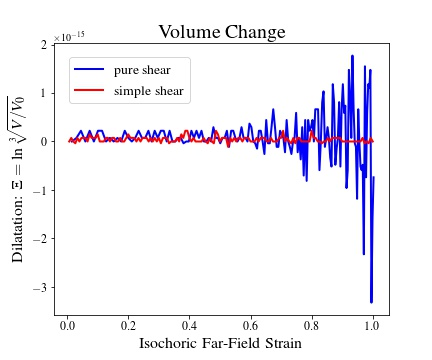
\includegraphics[width=10cm]{figures/isochoric.jpg}
	\caption{Response of a dodecahedron exposed to far-field motions of pure and simple shears.  Note that the ordinate is $\times 10^{-15}$ and machine precision is $\sim 2.2 \times 10^{-16}$.}
	\label{figIsochoric}
\end{figure}

\subsubsection{Geometric Strains}

How the thirty chords and the twelve irregular pentagons deform under far-field motions of pure shear is displayed in Fig.~\ref{figPureShears}.  Figure~\ref{figIsochoric} demonstrates that the overall response of a dodecahedron is isochoric during pure shear.  Regardless, Fig.~\ref{figPureShears} demonstrates that the individual chordal and pentagonal constituents deform in a non-homogeneous manner, where the strains have been calculated as geometric changes in dodecahedral shape.  This result agrees with in~vivo observations made by Perlman \& Bhattacharya \cite{PerlmanBhattacharya07} where confocal microscopy was used to image a breathing rat lung.

\begin{figure}
	\centering
	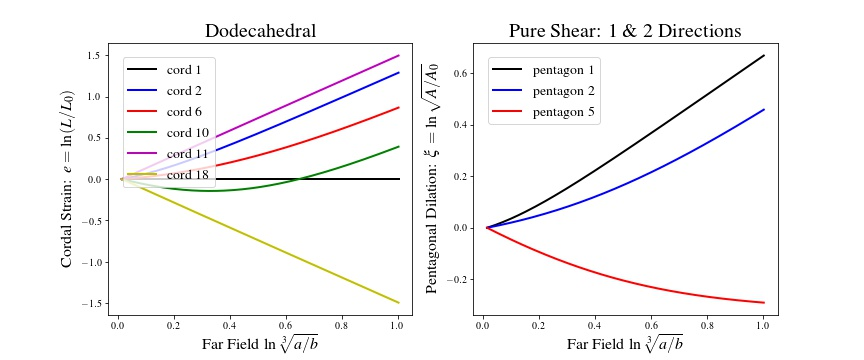
\includegraphics[width=14cm]{figures/squeeze12.jpg} \\
	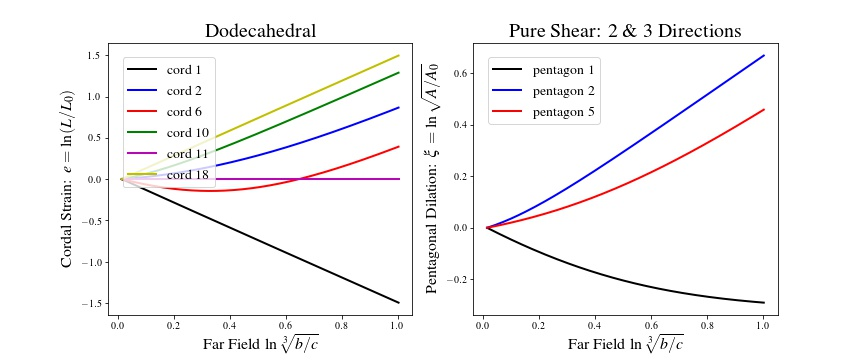
\includegraphics[width=14cm]{figures/squeeze23.jpg} \\
	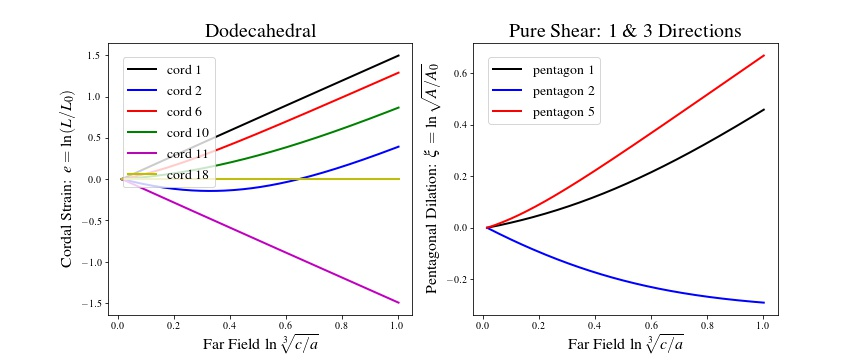
\includegraphics[width=14cm]{figures/squeeze13.jpg} 
	\caption{Response of a dodecahedron exposed to far-field pure-shear motions in the sense of Treloar \cite{Treloar75}: $a = \ell$, $b = 1/\ell$ and $c = 1$ in the top images; $a = 1$, $b = \ell$ and $c = 1/\ell$ in the middle images; and $a = 1/\ell$, $b = 1$ and $c = \ell$ in the bottom images, with $\ell$ denoting an elongation of extrusion.  In all six graphic images, the relevant (controlled) motion of the far-field pure shear is plotted along the abscissa.  In each image pair, the right graphic presents pentagonal dilations, while the left graphic presents chordal elongations. Only unique responses are plotted; repetitions are not.}
	\label{figPureShears}
\end{figure}

For the dodecahedral chords, there are six independent responses for motions of pure shear: two chords each for three of these lines, and eight chords each for the remaining three curves present in the left images of Fig.~\ref{figPureShears}.  For pentagons, there are three independent responses with four pentagons responding according to each curve shown in the right images.  Although different chords and pentagons deform differently when sheared in different directions, their collective responses are the same regardless of the far-field direction being sheared.  Consequently, the local geometric response of a dodecahedron is isotropic under the far-field motions of pure shear.  

How the thirty chords and the twelve irregular pentagons deform under far-field motions of simple shear is displayed in Fig.~\ref{figSimpleShears}.  Figure~\ref{figIsochoric} demonstrates that the overall response of a dodecahedron is isochoric during a far-field simple shear. Figure~\ref{figSimpleShears} demonstrates that the individual chordal and pentagonal constituents deform in a non-homogeneous manner during simple shears, like they do for pure shears.  However, unlike pure shears whose collective chordal and pentagonal responses remain isotropic, here they diverge from isotropy under motions of simple shear.  Simple shears in the 12 and 23 planes have the same collective response; whereas, simple shear in the 13 plane has a slightly different response.  

\begin{figure}
	\centering
	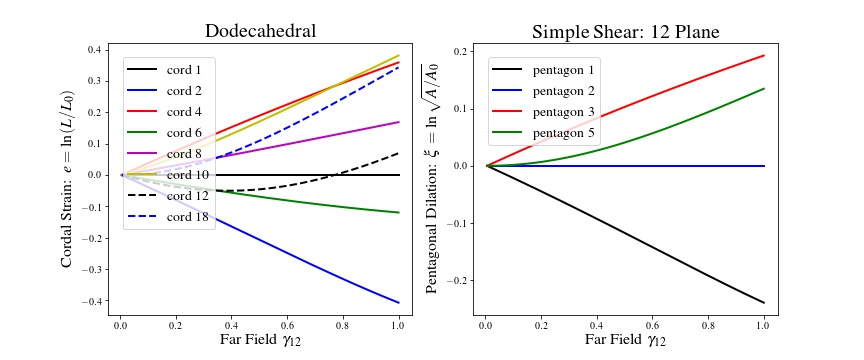
\includegraphics[width=14cm]{figures/shear12.jpg} \\
	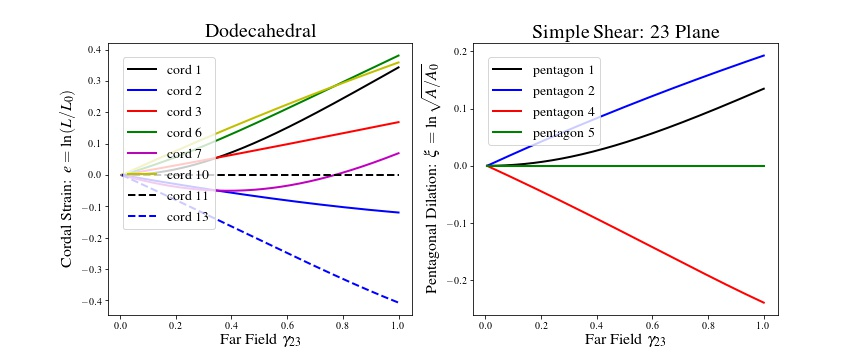
\includegraphics[width=14cm]{figures/shear23.jpg} \\
	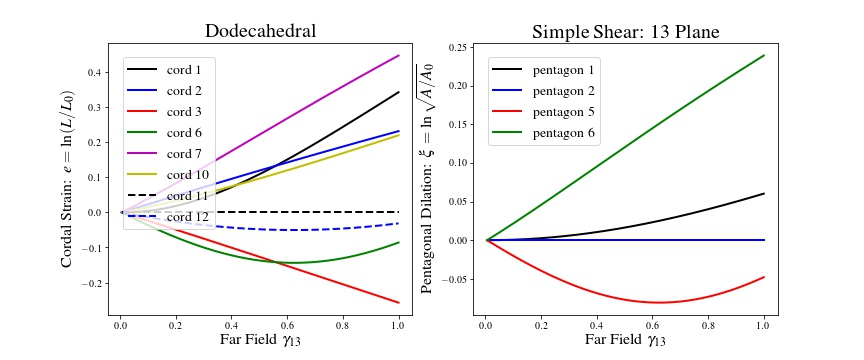
\includegraphics[width=14cm]{figures/shear13.jpg} 
	\caption{Response of a dodecahedron exposed to far-field simple-shear motions.  In all six graphic images, the relevant (controlled) motion of simple shear is plotted along the abscissa.  In each image pair, the right graphic presents pentagonal dilations, while the left graphic presents chordal elongations. Only unique responses are plotted; repetitions are not.}
	\label{figSimpleShears}
\end{figure}

Figures \ref{figDilatation}--\ref{figSimpleShears} establish that a dodecahedron is (nearly, but not completely) isotropic in its kinematic response, as measured by the geometric strains $e = \ln (L / L_0)$, $\xi = \ln \sqrt{A / A_0}$ and $\Xi = \ln \sqrt[3]{V / V_0}$.  Furthermore, even though a far-field deformation is homogeneous, in accordance with Conjecture~\ref{conjecture}, the local deformations within the individual constituents of an alveolus will typically be heterogeneous, which agrees with imaging data \cite{PerlmanBhattacharya07}.

\subsubsection{Thermodynamic Strains}

Addressing the septal response, modeled here as a set of twelve irregular pentagons per alveolus, we desire to come to a determination regarding how to best model the deformation occurring within these alveolar septa.  In the section above we investigated the geometric response of alveolar septa via the strain measure $\ln \sqrt{A/A_0}$, which quantifies dilation.  

The thermo\-dynamic strains arising from a Gram-Schmidt factorization of the deformation gradient put forward in \S\ref{secQR} specify three strain measures pertinent to a membrane: dilation $\xi = \ln \sqrt{ab/a_0 b_0}$, squeeze $\varepsilon = \ln \sqrt{ab_0 / a_0 b}$ and shear $\gamma = g - g_0$, where elongations $a$ and $b$ and magnitude of shear $g$ are illustrated in Fig.~\ref{figKinematics}.  Of these, dilation is an uniform response, while squeeze and shear describe non-uniform responses.  To acquire them requires knowing the deformation gradient.

The curves in Figs.~\ref{figPureShears} \& \ref{figSimpleShears} were obtained from geometric measures for chordal strain $\ln (L/L_0)$ and areal dilation $\ln \sqrt{A/A_0}$.  They were computed under separate conditions of pure and simple far-field shears.  The curves in Figs.~\ref{figPureShearsPentagons} \& \ref{figSimpleShearsPentagons} were obtained from thermo\-dynamic measures for membrane strain under the same far-field deformations.  The strains of dilation $\xi$, squeeze $\varepsilon$, and shear $\gamma$ were computed in accordance with \S\ref{secQR} using deformation gradients gotten from the pentagonal shape functions of Wachspress \cite{Wachspress75} discussed in \S\ref{secShapeFns}.\footnote{
	Five constant-strain triangles were also used to quantify the deformation gradient for each pentagonal surface at its centroid---the common vertex to all five triangles.  This approach provided accurate descriptions for uniform strain, i.e., dilation $\xi$, but not for the two non-uniform strains, viz., squeeze $\varepsilon$ and shear $\gamma$.
} 

\begin{figure}
	\centering
	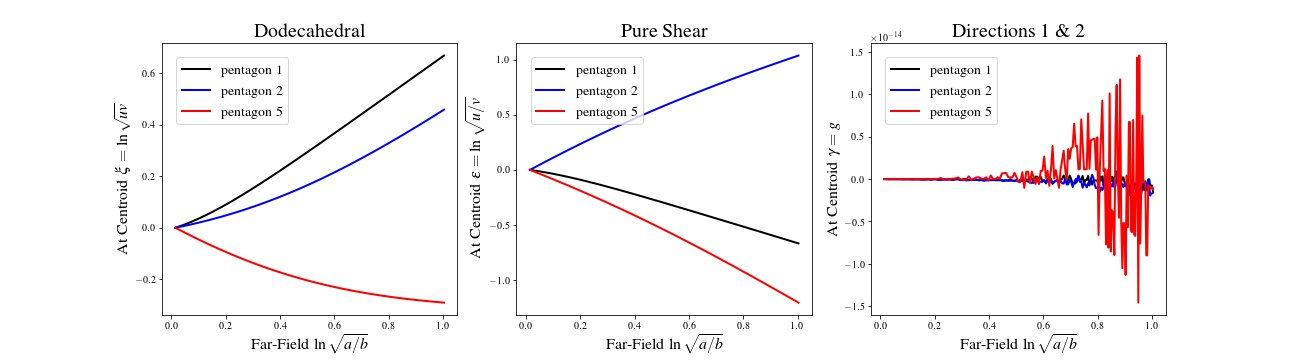
\includegraphics[width=\textwidth]{figures/pentagonalPureShear12.jpg} \\
	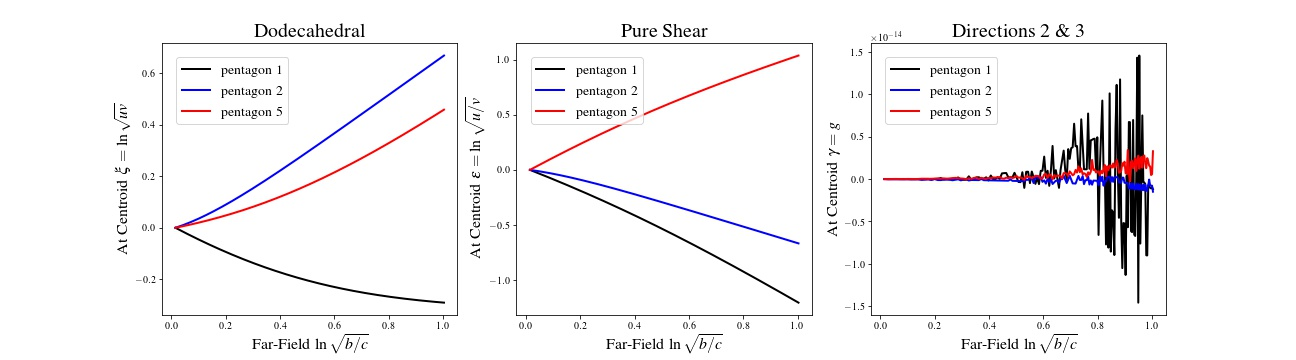
\includegraphics[width=\textwidth]{figures/pentagonalPureShear23.jpg} \\
	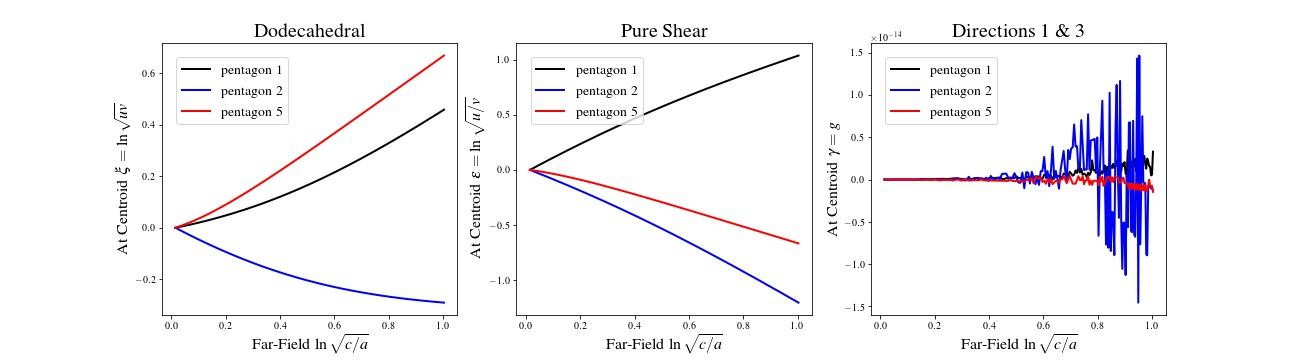
\includegraphics[width=\textwidth]{figures/pentagonalPureShear13.jpg} \\
	\caption{Same boundary conditions as in Fig.~\ref{figPureShears}.  Pentagonal areas were used to compute dilation in Fig.~\ref{figPureShears}.  The shape functions of Wachspress were used to compute dilation here.  The uniform response in the right column of Fig.~\ref{figPureShears} and in the left column above are the same, providing additional assurance that the code has been correctly implemented.  The squeeze response shown in the center column is the same for all three orientations of far-field pure shear, i.e., this response is isotropic.  The right column has ordinates scaled by $10^{-14}$ implicating that there is no simple shear response occurring within any pentagonal surface of the dodecahedron whenever it is subjected to a far-field motion of pure shear.}
	\label{figPureShearsPentagons}
\end{figure}

\begin{figure}
	\centering
	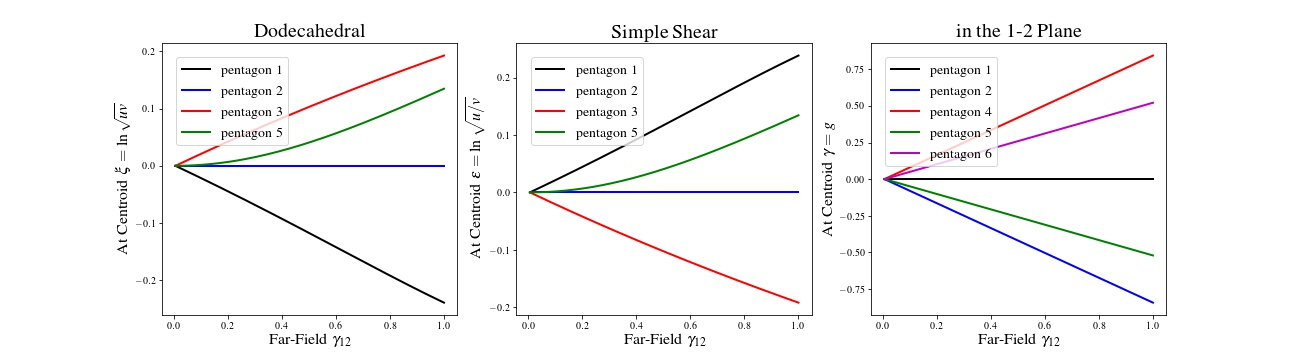
\includegraphics[width=\textwidth]{figures/pentagonalSimpleShear12.jpg} \\
	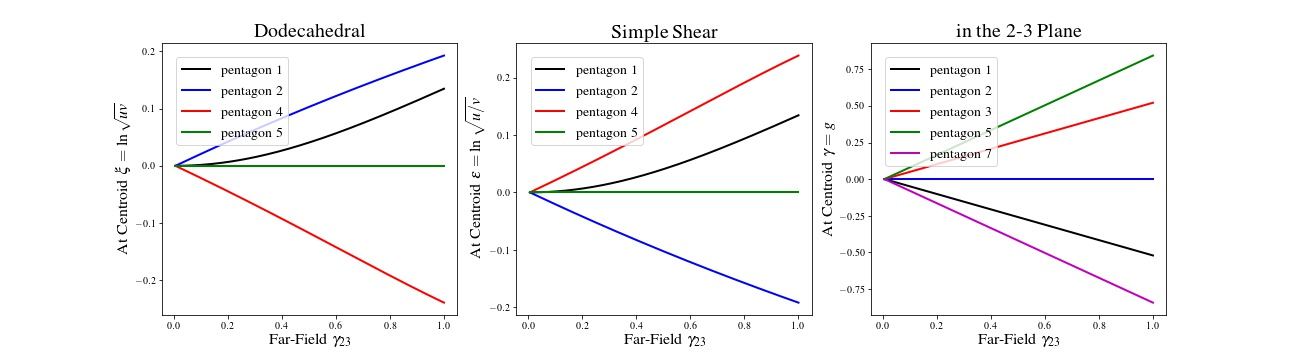
\includegraphics[width=\textwidth]{figures/pentagonalSimpleShear23.jpg} \\
	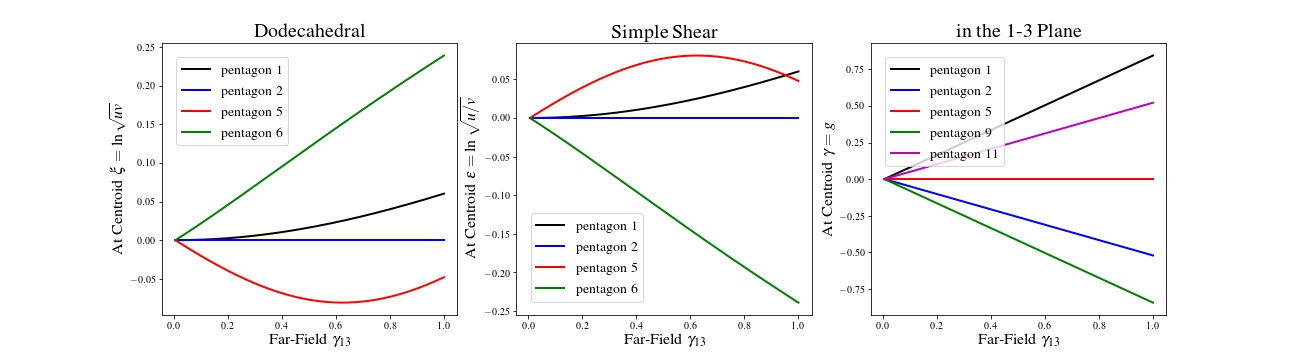
\includegraphics[width=\textwidth]{figures/pentagonalSimpleShear13.jpg} \\
	\caption{Same boundary conditions as in Fig.~\ref{figSimpleShears}.  Pentagonal areas were used to compute dilation in Fig.~\ref{figSimpleShears}.  The shape functions of Wachspress were used to compute dilation here. The uniform response in the right column of Fig.~\ref{figSimpleShears} and in the left column above are the same, providing additional assurance that the code has been correctly implemented.  Like the dilational responses of the left column, the squeeze responses of the center column are the same in the 1-2 and 2-3 planes, but differ in the 1-3 plane.  In all cases, the simple shear response of any pentagonal plane is proportional to that of the far-field shear imposed, further substantiating the code's implementation.  The shear response of the septal membranes is isotropic.}
	\label{figSimpleShearsPentagons}
\end{figure}

Figures~\ref{figPureShears}--\ref{figSimpleShearsPentagons} allow us to conclude that if septal dilation were the only mode of planar deformation thought to cause a mechanical response, then knowledge of the geometric strain $\xi = \ln \sqrt{A/A_0}$ would be adequate; there would be no need to introduce a separate finite-element discretization of the septal planes for acquiring their deformation gradients.  However, if the non-uniform responses of squeeze $\varepsilon$ and shear $\gamma$ are thought to contribute to the overall mechanical response of these membranes, then the shape functions of Wachspress \cite{Wachspress75,Wachspress16} ought to be used for acquiring the deformation gradient within a septal plane.  We found, but do not present figures to support this observation, that constant-strain triangles are not accurate enough for our application.  Strains derived from Wachspress shape functions are inhomogeneous; consequently, the deformation gradient will need to be evaluated at each Gauss point of integration within a pentagon, cf.\ \S\ref{secGauss}.

\subsection{Co-ordinate Pivoting}

The pivoting strategy of \S\ref{secRemedy} used to address the physical dilemma of \S\ref{secDilemma} did not engage often during our assessment of the code, but it did arise at least twice with effects illustrated in Figs.~\ref{figPivoting1} \& \ref{figPivoting3}.  Here one can see that there is a clear effect on the shear response within four pentagonal planes; however, no change is observed to have occurred in either the dilation or squeeze responses, as expected.  It is not always possible to know when or where a co-ordinate relabeling ought to occur; consequently, the algorithm put forward in \S\ref{secRemedy} is deemed necessary.

\begin{figure}
	\centering
	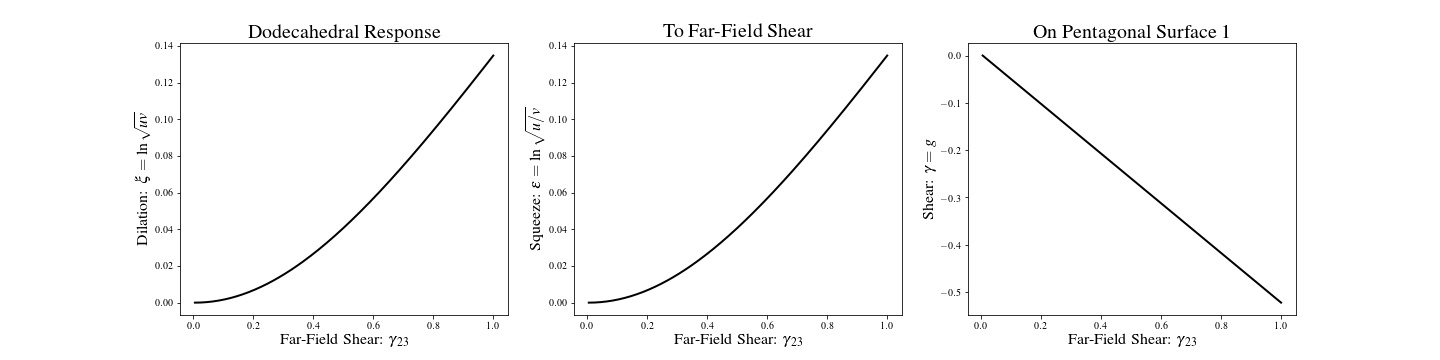
\includegraphics[width=\textwidth]{figures/continuousShearWithPivot1.jpg}
	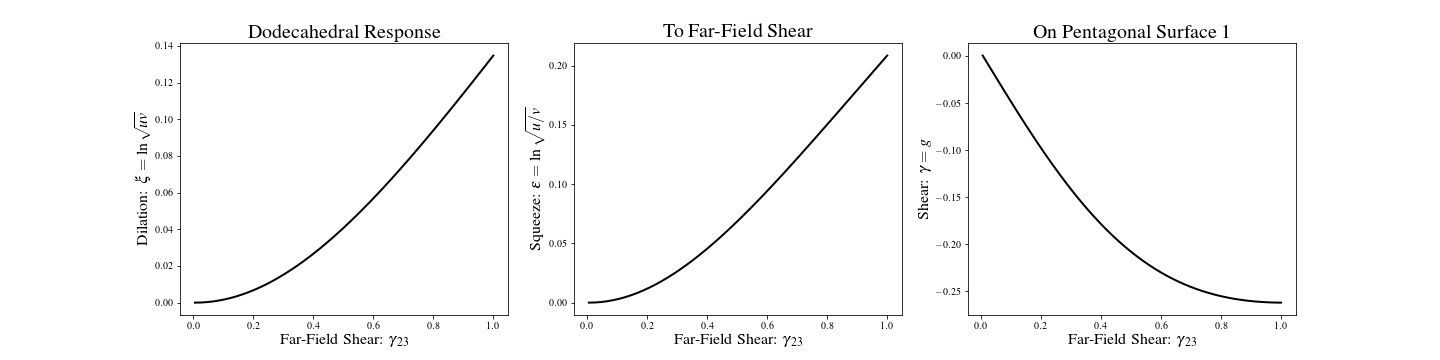
\includegraphics[width=\textwidth]{figures/continuousShearNoPivot1.jpg}
	\caption{A far-field shear of $\gamma_{23}$ is imposed on the dodecahedron.  Pentagons 1 and 8 exhibit the plotted response.  The top set of figures result whenever the pivoting strategy of \S\ref{secRemedy} is used, while the bottom set of figures result whenever no pivoting strategy is employed.  The dilation (left graphs) and squeeze (center graphs) responses are not effected by pivoting, only shear (right graphs) is effected.  Pivoting maintains a linear shear response under a far-field shearing of the dodecahedron, as desired.}
	\label{figPivoting1}
\end{figure}

\begin{figure}
	\centering
	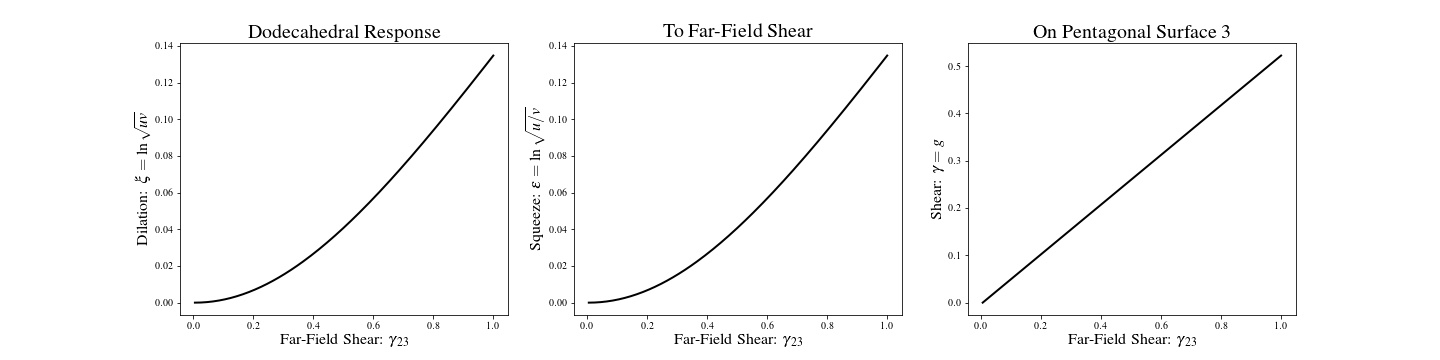
\includegraphics[width=\textwidth]{figures/continuousShearWithPivot3.jpg}
	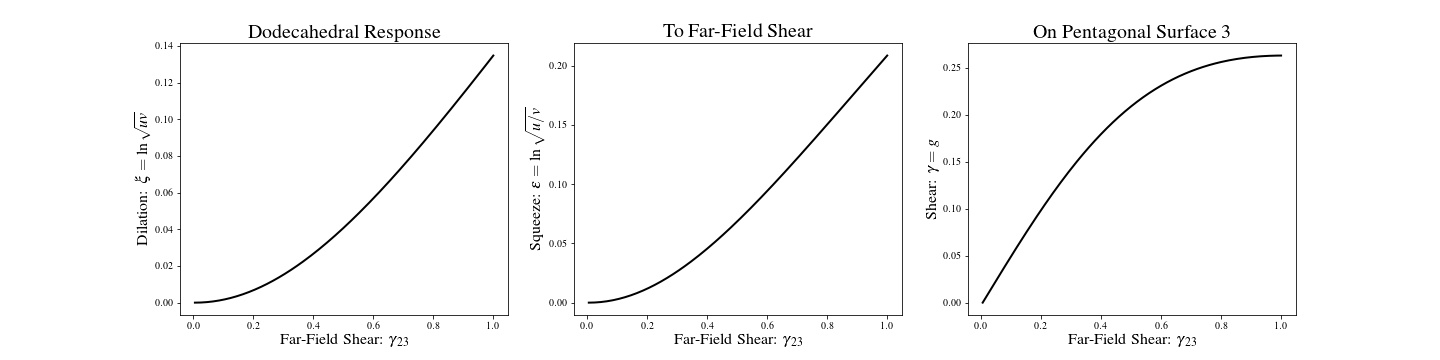
\includegraphics[width=\textwidth]{figures/continuousShearNoPivot3.jpg}
	\caption{A far-field shear of $\gamma_{23}$ is imposed on the dodecahedron.  Pentagons 3 and 10 exhibit the plotted response.  The top set of figures result whenever the pivoting strategy of \S\ref{secRemedy} is used, while the bottom set of figures result whenever no pivoting strategy is employed.  The dilation (left graphs) and squeeze (center graphs) responses are not effected by pivoting, only shear (right graphs) is effected.  Pivoting maintains a linear shear response under a far-field shearing of the dodecahedron, as desired.}
	\label{figPivoting3}
\end{figure}

\subsection{Compatible Membrane Deformations}

For a deformation to be compatible, and therefore integrable, the curl of its deformation gradient must vanish, viz., $\textrm{curl} (\mathbfsf{F}) = \textbf{0}$ \cite{Clayton15}. Equation~(\ref{compatibility}) provides constraint equations for the compatibility of planar motions, e.g., septal planes of an alveolus.  Here we test to make sure that these conditions are satisfied within the pentagonal planes of our alveolar dodecahedron, assuming that the shape functions of Wachspress apply.

Figure \ref{figCompatDilatation} presents the compatibility response at the centroid of a typical pentagonal plane during the uniform expansion of a regular dodecahedron out to 100\% strain.   Theoretically, all four derivatives should be zero for this motion. Actually, their values are on the order of machine precision.  Most importantly, whenever they are not zero, they lie along the $45^{\circ}$ diagonal, thereby verifying compatibility in the case of a dilatation.

\begin{figure}
	\centering
	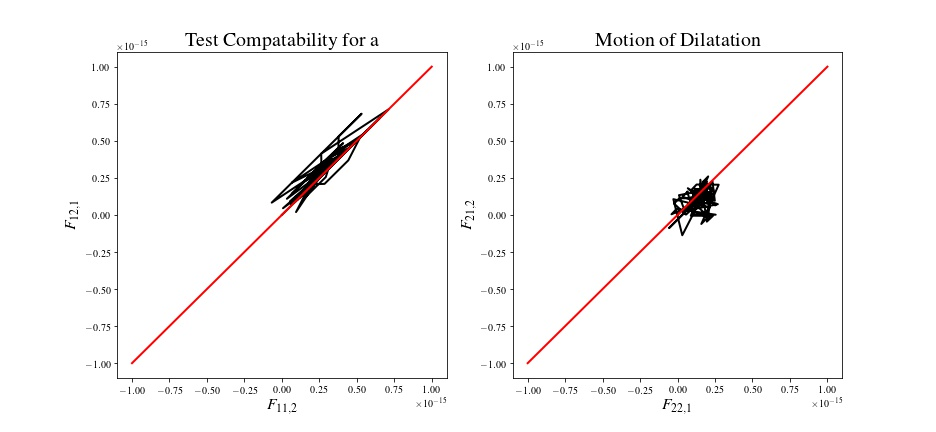
\includegraphics[width=\textwidth]{figures/compatibilityDilatation.jpg}
	\caption{Planar compatibility requires $F_{11,2} = F_{12,1}$ and $F_{22,1} = F_{21,2}$ where the left-hand sides are plotted as the absciss\ae\ and the right-hand sides are plotted as the ordinates.  For compatibility, the response ought to lie along the $45^{\circ}$ diagonal, which is drawn in red over the range of $\pm 10^{-15}$ where machine precision is about $2.2 \times 10^{-16}$.  Here the motion is one of uniform dilatation out to 100\% strain.}
	\label{figCompatDilatation}
\end{figure}

Similarly, Figs.~\ref{figCompatPureShearP5} \& \ref{figCompatSimpleShearP5} present typical responses for testing compatibility during far-field pure shear (Fig.~\ref{figCompatPureShearP5}) and simple shear (Fig.~\ref{figCompatSimpleShearP5}) deformations.  In both cases, one of the four pentagons around the girth of the dodecahedron (viz., \#5) has been selected, as both modes of deformation are activated in this pentagon.  In both cases, errors are typically less than ten times machine precision, thereby verifying compatibility in the cases of squeeze and shear.

\begin{figure}
	\centering
	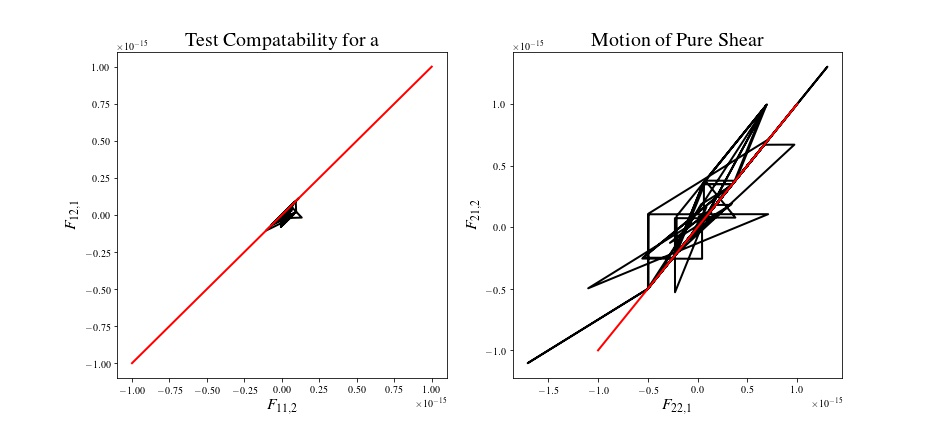
\includegraphics[width=\textwidth]{figures/compatibilityPureShearP5G7.jpg}
	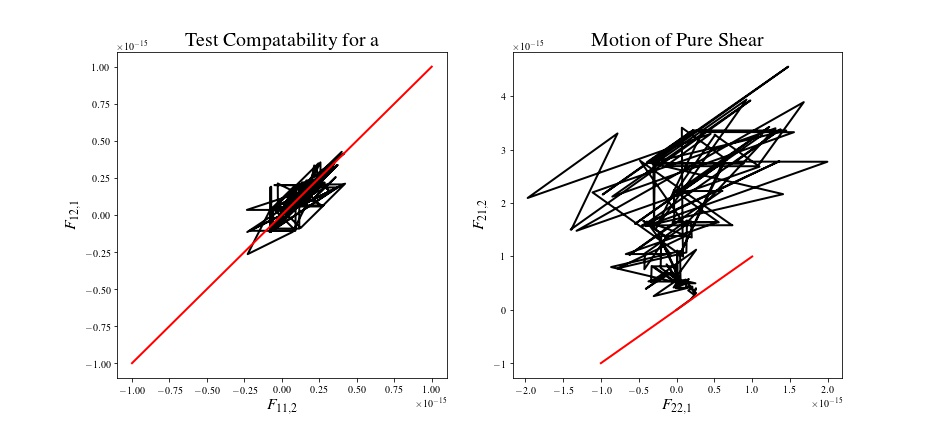
\includegraphics[width=\textwidth]{figures/compatibilityPureShearP5G5.jpg}
	\caption{Planar compatibility requires $F_{11,2} = F_{12,1}$ and $F_{22,1} = F_{21,2}$ where the left-hand sides are plotted as the absciss\ae\ and the right-hand sides are plotted as the ordinates.  For compatibility, the response ought to lie along the $45^{\circ}$ diagonal, which is drawn in red over the range of $\pm 10^{-15}$ where machine precision is about $2.2 \times 10^{-16}$.  Here the motion is one of pure shear out to 100\% strain with elongation occurring in the 1-direction, contraction occurring in the 2~direction, while the 3-direction is held fixed.  These results pertain to pentagon~5: nodes 15, 5, 12, 11, 1, cf.\ Fig.~\ref{figDodecahedron} and Table~\ref{TablePentagons}.  The top row of figures is the best response (at Gauss point 7, cf.\ Fig.~\ref{figQuadrature}) while the bottom row of figures is the worst response (at Gauss point 5).}
	\label{figCompatPureShearP5}
\end{figure}

\begin{figure}
	\centering
	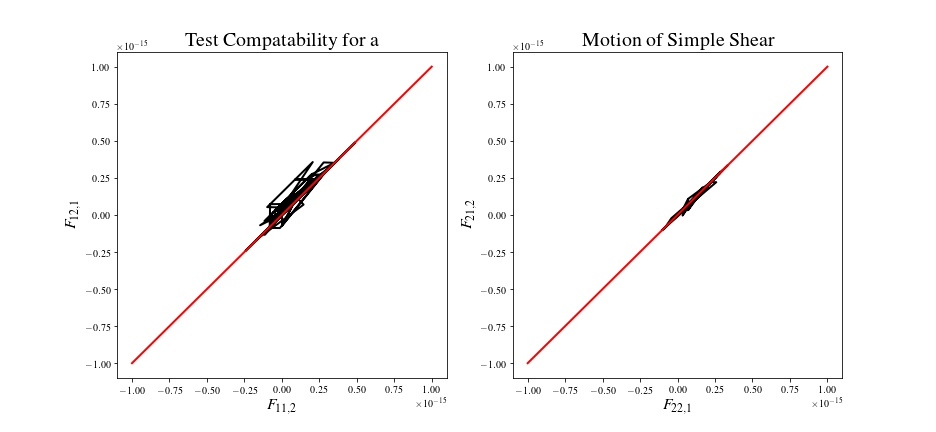
\includegraphics[width=\textwidth]{figures/compatibilitySimpleShearP5G7.jpg}
	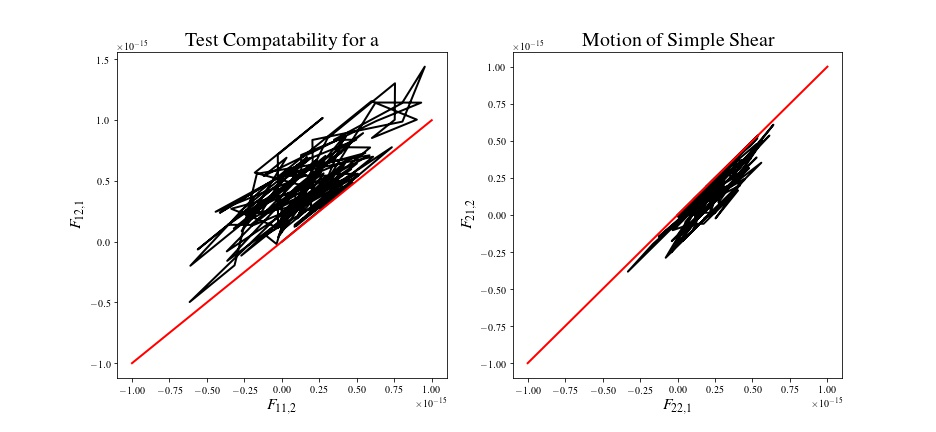
\includegraphics[width=\textwidth]{figures/compatibilitySimpleShearP5G5.jpg}
	\caption{Planar compatibility requires $F_{11,2} = F_{12,1}$ and $F_{22,1} = F_{21,2}$ where the left-hand sides are plotted as the absciss\ae\ and the right-hand sides are plotted as the ordinates.  For compatibility, the response ought to lie along the $45^{\circ}$ diagonal, which is drawn in red over the range of $\pm 10^{-15}$ where machine precision is about $2.2 \times 10^{-16}$.  Here the motion is one of simple shear out to 100\% strain, shearing along 1-2~planes in the 1-direction.  These results pertain to pentagon~5: nodes 15, 5, 12, 11, 1, cf.\ Fig.~\ref{figDodecahedron} and Table~\ref{TablePentagons}.  The top row of figures is the best response (at Gauss point 7, cf.\ Fig.~\ref{figQuadrature}) while the bottom row of figures is the worst response (at Gauss point 5).}
	\label{figCompatSimpleShearP5}
\end{figure}

This collective set of graphs, Figs.~\ref{figCompatDilatation}--\ref{figCompatSimpleShearP5}, investigate the constraint of compatibility in terms of the three fundamental modes of deformation: dilatation, squeeze and shear.  These figures verify that the constraint of compatibility is satisfied when using the pentagonal shape functions of Wachspress \cite{Wachspress75,Wachspress16} in our dodecahedral model, as errors are typically less than ten times machine precision.  This has been verified out to deformations that are at least three times those of their normal physiologic range.

Our kinematic analysis of a dodecaheron has been verified theoretically and numerically.

